\documentclass[mat1]{fmfdelo}
% \documentclass[fin1]{fmfdelo}
% \documentclass[isrm1]{fmfdelo}
% \documentclass[mat2]{fmfdelo}
% \documentclass[fin2]{fmfdelo}
% \documentclass[isrm2]{fmfdelo}

% naslednje ukaze ustrezno napolnite
\avtor{Marcel Čampa}

\naslov{Algoritem potisni-povišaj za iskanje maksimalnih pre\-to\-kov}
\title{Push-relabel algorithm for maximum flow problem}

% navedite ime mentorja s polnim nazivom: doc.~dr.~Ime Priimek,
% izr.~prof.~dr.~Ime Priimek, prof.~dr.~Ime Priimek
% uporabite le tisti ukaz/ukaze, ki je/so za vas ustrezni
\mentor{prof.~dr.~Sergio Cabello}
% \mentorica{}
% \somentor{}
% \somentorica{}
% \mentorja{}{}
% \mentorici{}{}

\letnica{2018} % leto diplome

%  V povzetku na kratko opišite vsebinske rezultate dela. Sem ne sodi razlaga organizacije dela --
%  v katerem poglavju/razdelku je kaj, pač pa le opis vsebine.
\povzetek{Ideja dela je spoznati se z osnovnimi pojmi teorije grafov, kot so omrežje, pretok in maksimalni pretok ter predstaviti algoritem potisni-povišaj za iskanje maksimalnega pretoka v omrežju. Algoritem je tudi implementiran, pokazana pa je tudi njegova časovna zahtevnost in pravilnost delovanja. Uporabnost iskanja maksimalnih pre\-to\-kov je ponazorjena z dvema primeroma iz vsakdanjega življenja.}

%  Prevod slovenskega povzetka v angleščino.
\abstract{The idea of this work is to get used to basic concepts of graph theory, e.g. network, flow and maximum flow. The core is an explanation of push-relabel algorithm for finding maximum flow through a network. The algorithm is also implemented and its time complexity and correctness are proven. It is also shown with two examples how one can use maximum flows in real life.}

% navedite vsaj eno klasifikacijsko oznako --
% dostopne so na www.ams.org/mathscinet/msc/msc2010.html
\klasifikacija{05C85, 68W05, 90C27, 90C35}
\kljucnebesede{pretok, potisni-povišaj, graf, omrežje, maksimalni pretok, opti\-mi\-za\-ci\-ja} % navedite nekaj ključnih pojmov, ki nastopajo v delu
\keywords{flow, push-relabel, graph, network, maximum flow, optimization} % angleški prevod ključnih besed

\zapisiMetaPodatke  % poskrbi za metapodatke in veljaven PDF/A-1b standard

% aktivirajte pakete, ki jih potrebujete
% \usepackage{tikz}
\usepackage{hhline}
\usepackage{float}
\usepackage{graphicx}
\usepackage[slovene]{babel}

% za številske množice uporabite naslednje simbole
\newcommand{\R}{\mathbb R}
\newcommand{\N}{\mathbb N}
\newcommand{\Z}{\mathbb Z}
\newcommand{\C}{\mathbb C}
\newcommand{\Q}{\mathbb Q}

% matematične operatorje deklarirajte kot take, da jih bo Latex pravilno stavil
% \DeclareMathOperator{\conv}{conv}

% vstavite svoje definicije ...
%  \newcommand{}{}

\begin{document}

\section{Uvod}

Tema mojega diplomskega dela je algoritem potisni-povišaj, s katerim iščemo maksimalni pretok v danem pretočnem omrežju. V angleščini rečemo temu algoritmu \textit{push-relabel algorithm}, zato se marsikomu morda porodi vprašanje,
zakaj prevod \textit{relabel} v \textit{povišaj}. Za ta prevod sem se odločil zato, ker takrat, ko opravimo tako imenovano operacijo \textit{relabel}, vozlišče postavimo na večjo višino.

Cilj tega dela je spoznati se z osnovnimi koncepti teorije grafov in kombinatorične optimizacije, predvsem pa se od bližje spoznati z enim od učinkovitejših algorimov za iskanje maksimalnega pretoka. Poleg našega algoritma
sodijo med bolj znane še algoritem Forda in Fulkersona, Edmonds-Karpov algoritem, Dinicev algoritem, KRT (King, Rao, Tarjan) in KRT+O (KRT + Orlin). Prva dva algoritma imata slabšo časovno zahtevnost od algoritma potisni-povišaj,
Dinicev ima enako kot osnovna verzija potisni-povišaj, zadnja dva pa sta hitrejša.

Ko sem se udomačil v teoriji algoritma, sem se lotil implementacije v programskem jeziku C++, ki sem ga izbral povsem arbitrarno. Največjo vlogo pri izbiri sta sicer igrali hitrost in praktičnost, vendar sem se za C++ odločil, ker v njem
že dolgo časa nisem napisal ničesar. Med pisanjem algoritma sem pravzaprav čisto sam ,,odkril'' izboljšavo algoritma, ki izboljša časovno zahtevnost navadnega potisni-povišaj z $\mathcal{O}(V^2E)$ na $\mathcal{O}(V^3)$, kjer je $V$ število vozlišč
v omrežju, $E$ pa število povezav. Časovne zahtevnosti izboljšave ne bomo dokazovali, nekaj podobnega pa se najde v knjigi \cite{clrs}.

Sedaj, ko je bil algoritem implementiran in stestiran, sem kolebal med tem, ali naj algoritem poženem na primerih različne velikosti in ugotovitve vključim v to delo, ali pa naj raje predstavim, kako nam lahko maksimalni pretoki pomagajo
v vsakdanjem življenju. Vsekakor se mi je zdela bolj poučna slednja stvar, zato sem se zanjo tudi odločil. Navsezadnje je tudi zanimivejša kakor suhoparno nabijanje številk v tabelo, ki je sama sebi namen.

\section{Osnovne definicije}

V tem razdelku se bomo najprej spoznali z osnovnimi definicijami teorije grafov, brez katerih ne bomo mogli. Definicije so vzete iz knjig \cite{clrs, uvtg}, nekatere pa so malce spremenjene. Nato si bomo pogledali manj znane definicije in definicije specifične za algoritme tipa \textit{potisni-povišaj}.

\begin{definicija}
\textbf{Graf} $G$ je par množic $G = (V,E)$, kjer je $V$ množica vozlišč grafa, $E \subseteq V \times V$ pa je množica usmerjenih povezav grafa $G$.
\end{definicija}

\begin{definicija}\label{def:omrezjeprepustnost}
Naj bo $G = (V, E)$ graf. \textbf{Omrežje} na grafu $G$ je par $(G, c)$, kjer je $c \colon V \times V \rightarrow \mathbb{R}^+_0 \cup \{\infty\}$ \textbf{funkcija prepustnosti}, ki vsakemu paru vozlišč $(u,v)$ priredi prepustnost $c(u,v)$ povezave od $u$ do $v$. Prepustnost $c(u,v)$ je enaka $\infty$ natanko tedaj, ko prepustnost povezave ni omejena.

Velja še, da $c(u,v)=0$ natanko tedaj, ko povezava ne obstaja v $G$.
\end{definicija}

\begin{opomba}
Prepustnosti povezave bomo dostikrat rekli \textit{kapaciteta} povezave.
\end{opomba}

\begin{definicija}
Naj bo $G = (V,E)$ graf in $(G,c)$ omrežje na grafu $G$. \textbf{Pretočno omrežje} na omrežju $(G,c)$ je četverica $(G,c,s,t)$, kjer je $s\in V$ začetno vozlišče pretočnega omrežja, rečemo mu \textbf{izvir}, $t\in V$ pa končno vozlišče pretočnega omrežja, ki mu pravimo \textbf{ponor}.
\end{definicija}

\begin{definicija} \label{def:psevdopretok}
\textbf{Psevdopretok} je funkcija $f \colon V \times V \rightarrow \mathbb{R}$, ki zadošča pogojema:
\begin{enumerate}
\item Za vsaki vozlišči $u,v \in V$ velja $f(u,v) = - f(v,u)$.
\item Za vsaki vozlišči $u,v \in V$ velja $f(u,v) \leq c(u,v)$, kjer je $c$ funkcija pre\-pu\-stno\-sti.
\end{enumerate}
\end{definicija}

\begin{definicija}\label{def:resprepustnost}
\textbf{Residualna prepustnost} povezave glede na trenuten pse\-vdo\-pre\-tok $f$ je funkcija $c_f \colon V \times V \rightarrow \mathbb{R}^+_0 \cup \{\infty\}$, definirana kot razlika prepustnosti povezave in trenutnega toka preko nje. Velja torej $c_f(u,v) = c(u,v) - f(u,v)$.
\end{definicija}

\begin{definicija}
  Naj bo $G = (V,E)$ pretočno omrežje in $f$ tok v tem omrežju. \textbf{Residualno omrežje} omrežja $(G,c,s,t)$, inducirano s tokom $f$, je $G_f = (V,E_f)$, kjer je \[ E_f = \{ (u,v) \in V \times V \mid c_f(u,v) > 0 \}. \]
\end{definicija}

\begin{opomba}
  Opazimo dve stvari. O grafu $G$ smo govorili kot o pretočnem omrežju. To storimo takrat, ko nas $c$, $s$ in $t$ ne zanimajo, ali pa je iz konteksta razvidno, kaj so. Druga stvar pa je, da smo uporabili besedo \textit{tok}, brez predhodne definicije le-tega.
  Za sedaj si lahko mislimo, da je to psevdopretok, kar je povsem smiselno v kontekstu algoritma potisni-povišaj.
\end{opomba}

\begin{definicija}\label{def:presezek}
\textbf{Presežek} za psevdopretok $f$ je funkcija $e_f \colon V \rightarrow \mathbb{R}$, definirana z $e_f(u) = \frac{1}{2}\left(\sum_{v \in V} f(v,u) - \sum_{v \in V} f(u,v)\right)$. Če je $e_f(u) > 0$, pravimo, da je $u$ \textbf{v presežku}.
\end{definicija}

\begin{opomba}
  V formuli za $e_f(u)$ iz definicije \ref{def:presezek} je faktor $\frac{1}{2}$ zato, ker po definiciji psevdopretoka (definicija \ref{def:psevdopretok}) zaradi asimetrije v formuli za $e_f(u)$ tako vse tokove štejemo dvakrat.
\end{opomba}

Z drugimi besedami bi lahko rekli, da funkcija $e_f$ za vsako vozlišče pove, koliko preveč toka je vanj priteklo. To je ravno razlika med vsoto pritečenih tokov in vsoto odtečenih tokov.

\begin{opomba}
  Notacija $e_f$ za presežek je bolj stroga oblika notacije $e$. Ko nas $f$ ne bo zanimal, ali pa bo iz konteksta razviden, bomo pisali samo $e$.
\end{opomba}

\begin{definicija}
\textbf{Predpretok} $f$ je tak psevdopretok, v katerem za vsak $v \in V \setminus\{s\}$ velja, da je neto tok, ki priteče v vozlišče $v$, nenegativen, torej da velja $e_f(v) \geq 0$.
\end{definicija}

\begin{definicija}
\textbf{Pretok} $f$ je tak psevdopretok, v katerem za vsak $v \in V \setminus\{s,t\}$ velja, da je neto tok, ki priteče v vozlišče $v$, enak nič, torej da velja $e_f(v) = 0$.
\end{definicija}

Algoritmi tipa potisni-povišaj namreč ne ohranjajo Kirchoffovega zakona\footnote{Kirchoffov zakon pove, da je vsota tokov, ki pritečejo v vozlišče $u$, enaka vsoti tokov, ki iz vozlišča $u$ odtečejo, torej $\sum_{v\in V} f(v,u) = \sum_{v\in V} f(u,v)$. V našem primeru za vsako vozlišče $u \in V \setminus \{s\}$ velja $\sum_{v\in V} f(v,u) \geq \sum_{v\in V} f(u,v)$.}, ki velja za pretok. Zato pri algoritmih tega tipa govorimo o predpretoku. Ker ne ohranjajo Kirchoffovega zakona, definiramo naslednjo funkcijo.

\begin{definicija}
\textbf{Vrednost pretoka} $f$ je tok, ki vstopa v ponor $t$. Označimo ga z $|f|$. Velja torej $|f| = e_f(t)$.
\end{definicija}

\begin{definicija}
\textbf{Maksimalni pretok} je pretok $f$, za katerega velja \[|f| = \max_{f_i} |f_i|,\] kjer $f_i$ teče po vseh možnih pretokih skozi omrežje.
\end{definicija}

\begin{opomba}
  Maksimalni pretok obstaja vedno, lahko pa se zgodi, da je $|f| = \infty$ (v primeru, ko obstaja \textit{pot} iz $s$ v $t$, na kateri imajo vse povezave neomejeno kapaciteto)
  ali da je $|f| = 0$ (v primeru, ko ni \textit{poti} iz $s$ v $t$).
\end{opomba}

Naslednja definicija nam bo dala nov atribut vozlišč.

\begin{definicija}\label{def:visinska_funkcija}
Naj bo $G=(V,E,s,t)$ pretočno omrežje. \textbf{Višinska funkcija} je funkcija $h\colon V \rightarrow \N_0$, za katero velja
\begin{enumerate}
\item $h(s) = |V|$ in $h(t) = 0$,
\item $h(u) \leq h(v) + 1$, za vsako povezavo $(u,v) \in E_f$, kjer je $E_f$ množica povezav v residualnem grafu $G_f$.
\end{enumerate}
\end{definicija}

\begin{opomba}
Privzeli bomo, da če v grafu obstaja povezava $(u,v)$, potem ne obstaja povezava $(v,u)$. Privzeli bomo tudi, da v omrežju nimamo povezav v izvir $s$ in nimamo povezav iz ponora $t$.
\end{opomba}







\section{Iskanje maksimalnega pretoka z algoritmom potisni-povišaj}

V tem razdelku si bomo podrobneje ogledali algoritem \textit{potisni-povišaj}. Začeli bomo s kratkim opisom delovanja algoritma in intuitivno razložili, kako algoritem deluje. Nato si bomo pogledali psevdokodo algoritma in se z njo pobližje spoznali na zgledu. Sledila bo implementacija algoritma z rahlo izboljšavo v programskem jeziku C++. Pokazali bomo pravilnost delovanja algoritma in njene implementacije ter časovno zahtevnost algoritma.

\subsection{O algoritmu}
Algoritem potisni-povišaj deluje po preprostem principu iz na\-ra\-ve. Predsavljajmo si, da imamo rečno omrežje, ki se začne v eni točki in konča v eni točki. Z drugimi besedami imamo eno reko, ki pa se vmes poljubno deli in združuje. Seveda je na Zemlji prisotna gravitacijska sila, ki povzroči, da voda teče od višje točke proti nižji, recimo od izvira v hribih do ponora v morje, vmes pa ubira tako pot, da nikjer ne gre navzgor. V jeziku grafov lahko predstavimo omenjeni pojav na naslednji način. Tam, kjer se reka deli oziroma združi, postavimo vozlišče grafa. Del reke med dvema razvejiščema predstavlja povezavo med razvejiščema pripadajočima vozliščema. Izvir in ponor reke predstavljata vozlišči $s$ in $t$. Vsakemu vozlišču pripišemo višino, na kateri se nahaja, in količino vode, ki je vanj pritekla in odtekla. Seveda se v naravi ne zgodi (razen v primeru neurij), da bi v razvejišče priteklo več vode, kot pa je je iz njega odteklo. Prav tako ne more priteči manj vode, kot je odteče.

Sedaj, ko smo se spomnili, kako deluje mati narava, in to prevedli v matematični jezik, si podrobneje poglejmo, kako deluje algoritem potisni-povišaj. Začnemo z omrežjem (od sedaj bomo rajši kot o grafih govorili o omrežjih) $G = (V, E, s, t)$ in funkcijama $c\colon V \times V \rightarrow \N_0$, ki vsaki povezavi priredi njeno kapaciteto, in $f\colon V \times V \rightarrow \Z$, ki za vsako povezavo pove, koliko vode teče v nekem trenutku preko nje. Vozliščem $v \in V$ priredimo še funkciji $h\colon V \rightarrow \N_0$, ki določa višino vozlišča, in $e\colon V \rightarrow \N_0$, ki pove, koliko preveč vode je priteklo v neko vozlišče.\footnote{Tu smo za kodomene vzeli $\N_0$ oziroma $\Z$ namesto različic z $\R$ iz definicij. Tega nam ni bilo potrebno storiti, vendar se bomo v nadaljevanju ukvarjali s celoštevilskimi vrednostmi, v definicijah pa je še vseeno smiselno pisati, da so stvari definirane na realnih številih.} Seveda velja \[e(u) = \frac{1}{2}\left(\sum_{v \in V} f(v,u) - \sum_{v \in V} f(u,v)\right).\] Algoritem na začetku nastavi višino vseh vozlišč razen vozlišča $s$ na nič in višino $s$ na $|V|$. Tako na začetku velja $h(s) = |V|$ in $h(u) = 0$, $u \in V \setminus \{s\}$. Nato potisnemo iz $s$ tok v sosednja vozlišča tako, da zasičimo povezave, torej da velja $f(s, v) = c(s, v)$, za vse $v \in V$. Poleg tega dodamo v residualno omrežje še obratne povezave, katerim nastavimo $f(v,s) = -f(s,v)$, da zadostimo pogoju (1) iz definicije psevdopretoka (definicija \ref{def:psevdopretok}). S tem smo ustvarili tako imenovani \textit{predpretok}. To smo lahko storili, ker je višina vozlišča $s$ večja kot višina sosednjih vozlišč $v$, saj $h(s) = |V| > 0 = h(v)$.

Rezultat te operacije je, da se je v vozliščih, sosednjih vozlišču $s$, nabrala odvečna voda. Za ta vozlišča torej velja $e(v) > 0$. Sedaj lahko potisnemo vodo iz teh vozlišč naprej, saj je vode v njih preveč, želimo pa, da je odteče toliko, kot je priteče. Vendar tega ne moremo storiti, saj so višine sosednjih vozlišč prav tako enake nič. Zato si izberemo neko vozlišče $u$, v katerega je priteklo preveč vode, in mu povečamo višino na $\min\{h(v) : (u,v) \in E_f\} + 1$. S tem smo omogočili, da bo voda odtekla v vsaj eno izmed vozlišč. Ta postopek ponavljamo, dokler lahko potisnemo tok v omrežju ali pa povišamo neko vozlišče. Tok, ki na koncu priteče v $t$, je enak maksimalnemu pretoku omrežja, kar bomo pokazali kasneje.\\

Oglejmo si sedaj psevdokodo algoritma, ki je malce spremenjena kot psevdokoda v \cite{clrs}. Spoznali smo, da je algoritem sestavljen iz dveh osnovnih operacij, \textit{potiskanja} in \textit{povišanja}, zato se posvetimo tema operacijama. Začnimo s potiskanjem.\\

\begin{verbatim}
POTISNI (u, v)
1   // Potisnemo lahko, če je e(u) > 0,
2   // c_f(u,v) > 0 in h(u) = h(v) + 1.
3   delta = min{ e(u), c(u,v) - f(u,v) }
4   f(u,v) += delta
5   f(v,u) -= delta
6   e(u) -= delta
7   e(v) += delta
\end{verbatim}~

To operacijo lahko storimo, če ima $u$ presežek toka, torej, če velja $e(u) > 0$, če je residualna kapaciteta povezave $c_f(u,v) > 0$ in če sta vozlišči $u$ in $v$ na primernih višinah, torej če velja $h(u) = h(v) + 1$. Najprej izračunamo, kolikšno količino $\delta$ lahko potisnemo. Ta je enaka minimumu med presežkom toka v vozlišču $u$ in residualno kapaciteto povezave, ki je enaka $c(u,v) - f(u,v)$. To storimo v vrstici 3. V vrsticah 4 in 5 potisnemo tok $\delta$ po povezavi $(u,v)$ in tok
$-\delta$ po obratni povezavi. V vrsticah 6 in 7 posodobimo še presežek toka v krajiščih povezave. To storimo tako, da v začetnem vozlišču presežek zmanjšamo za tok, ki smo ga potisnili, v končnem vozlišču pa presežek povečamo.

Nadaljujmo z operacijo povišanja vozlišča.\\

\begin{verbatim}
POVIŠAJ (u)
1   // Vozlišče u povišamo, če je e(u) > 0 in
2   // za vsak v iz V, (u,v) v E_f, velja h(u) <= h(v).
3   h(u) = min{ h(v) : (u,v) v E_f } + 1
\end{verbatim}~

Operacija povišanja vozlišča $u$ je precej enostavna. Storimo jo takrat, ko ima vozlišče $u$ presežek toka, torej velja $e(u) > 0$, a hkrati ne moremo potisniti toka v sosednja vozlišča, saj so vsa na večji ali enaki višini kot $u$.

V opisu algoritma smo navedli še \textit{inicializacijo predpretoka}. Zapišimo psevdokodo za to operacijo.\\

\begin{verbatim}
INICIALIZIRAJ_PREDPRETOK(G,s)
 1   // V grafu G z izbranim izvirom s
 2   // inicializiramo predpretok.
 3   ZA vsak v v V(G)
 4       h(v) = 0
 5       e(v) = 0
 6   ZA vsak (u,v) v E(G)
 7       f(u,v) = 0
 8   h(s) = |V|
 9   ZA vsak v, za katerega obstaja (s,v) v E(G)
10       f(s,v) = c(s,v)
11       f(v,s) = -f(s,v)
12       e(v) = f(s,v)
\end{verbatim}~

Kot smo dejali, zgornja operacija nastavi višine vozlišč, tok po povezavah in presežek toka v vozliščih na nič. To storimo v vrsticah 3--7. V vrstici 8 nato nastavimo višino vozlišča $s$ na število vseh vozlišč v omrežju, torej $h(s) = |V|$. V vrsticah 10 in 11 nato potisnemo tok prek vseh povezav, ki izhajajo iz $s$, in posodobimo tok po obratnih povezavah. V vrstici 12 nato popravimo še presežek toka v vozliščih, ki so sosednja $s$. Opazimo, da nismo odšteli presežka toka v vozlišču na začetku povezave, torej v vozlišču $s$. Tega nismo storili, ker je to nepotrebno; predstavljamo si namreč, da je v vozlišču $s$ lahko poljubna količina vode, več kot je potrebujemo, več je lahko dobimo. Kasneje bomo videli, kaj se zgodi, če smo v inicializaciji predpretoka poslali preveč vode, kot je omrežje lahko spusti skozi.

Čas je, da navedemo še glavni del algoritma, torej ,,program'', ki uporablja zgoraj navedene operacije. Psevdokoda je na videz precej preprosta.\\

\begin{verbatim}
POTISNI-POVIŠAJ(G,s)
1   INICIALIZIRAJ_PREDPRETOK(G,s)
2   DOKLER obstaja mogoča operacija POTISNI ali POVIŠAJ
3       izvedi mogočo operacijo
\end{verbatim}~

Na videz nedolžna, vendar skriva rahlo prepreko do povsem direktne im\-ple\-men\-ta\-ci\-je. Vprašanje, ki se pojavi, je namreč, kako vedeti, ali lahko potisnemo oziroma po\-vi\-ša\-mo. Na to vprašanje bomo odgovorili v nadaljevanju. Oglejmo si najprej zgled delovanja algoritma in sproti se nam morda porodi ideja.\\

\subsection{Primer delovanja algoritma}

Vzemimo preprosto omrežje na petih vozliščih. Pet vozlišč smo izbrali zato, ker je to najmanjše število vozlišč, pri katerem se lahko dogajajo zanimive reči. Naj velja $G = (V, E, s, t)$, kjer je
\begin{align*}
	V &= \{0,1,2,3,4\},\\
	E &= \{(0,1), (0,2), (2,1), (1,3), (1,4), (3,4)\},\\
	s &= 0,\\
	t &= 4.
\end{align*}
Kapacitete povezav so podane v naslednji tabeli.

\begin{table}[h!]
\centering
\caption{Kapacitete povezav omrežja $G$.}
\begin{tabular}{|l|c|c|c|c|c|c|}
\hline
         & $(0,1)$ & $(0,2)$ & $(2,1)$ & $(1,3)$ & $(1,4)$ & $(3,4)$\\ \hline
$c(u,v)$ &   $10$  &   $6$   &   $4$   &   $8$   &   $5$   &   $4$  \\ \hline
\end{tabular}
\end{table}~

Omrežje $G$ na začetku izgleda takole:

\begin{figure}[H]
  \centering
  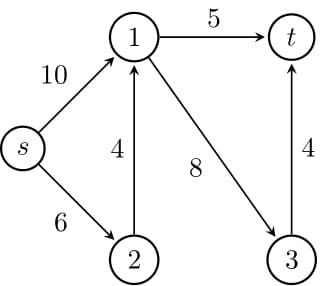
\includegraphics[scale=.358]{images/graf2-1/graf2-1-1.jpg}
  \caption{Pretočno omrežje, ki ga bomo uporabili kot zgled delovanja algoritma potisni-povišaj.}
\end{figure}

Poiščimo sedaj maksimalni pretok skozi to omrežje s pomočjo zgoraj opisanega algoritma potisni-povišaj.
Zaradi večje preglednosti residualnih povezav ne bomo risali, privzemimo pa, da če na povezavi $(u,v)$ teče tok $f(u,v)$,
obstaja residualna povezava $(v,u)$ kapacitete $c(v,u) = 0$, po kateri teče tok $f(v,u) = -f(u,v)$.\footnote{Stvar na prvi
pogled izgleda malce čudno, vendar če se spomnimo definicij \ref{def:omrezjeprepustnost}, \ref{def:psevdopretok} in \ref{def:resprepustnost}, vidimo,
da se stvari ujemajo, saj $c, c_f \colon V \times V \rightarrow \R^+_0 \cup \{\infty\}$ in $c_f(v,u) = c(v,u) - f(v,u) = 0 - (-f(u,v)) = f(u,v) \geq 0$.}

Najprej inicializiramo predpretok. Višino in presežek toka v vseh vozliščih na\-sta\-vi\-mo na $0$ in vsaki povezavi
damo tok $0$. Nato višino vozlišča $s$ nastavimo na $|V| = 5$ in vsaki povezavi, ki se začne v $s$, torej
povezavi $(0,1)$ in $(0,2)$, zasičimo. Na koncu še posodobimo presežek toka v vozliščih, sosednjim vozlišču $s$.
Omrežje sedaj izgleda tako:

\begin{figure}[H]
  \centering
  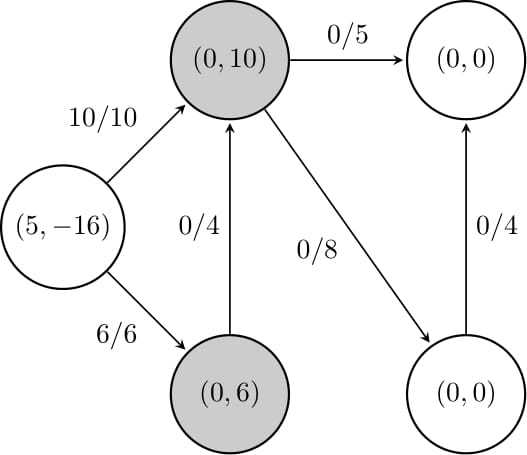
\includegraphics[scale=.358]{images/graf2-2/graf2-2-1.jpg}
  \caption{Pretočno omrežje po inicializaciji predpretoka. Par $(h, e)$ v vozlišču $u$ določa trenutno višino vozlišča $h(u)$ ter njegov presežek toka $e(u)$. Sivo obarvani sta vozlišči v presežku. Par $f/c$ na povezavi določa, kolikšen tok $f$ teče po tej povezavi in kolikšna je prepustnost povezave ($c$).}
\end{figure}

Sedaj imamo dve vozlišči v presežku, vendar iz nobenega ne moremo potisniti toka. Zato povišamo vozlišče $1$ na $\min \{h(0), h(3), h(4)\} + 1 = \min \{5, 0, 0\} + 1 = 1$. Sedaj lahko iz vozlišča $1$ tok potisnemo.
Po povezavi $(1,4)$ lahko pošljemo $\delta = \min\{e(1), c(1,4) - f(1,4)\} = c(1,4) - f(1,4) = 5 - 0 = 5$ enot in s tem zasičimo povezavo. V vozlišču nam ostane še $e(1) = 5$. Sedaj pošljemo po povezavi
$(1,3)$ $\delta = \min \{e(1), c(1,3) - f(1,3)\} = 5$ enot. Posodobimo $f$ in $e$ in dobimo naslednje stanje.

\begin{figure}[H]
  \centering
  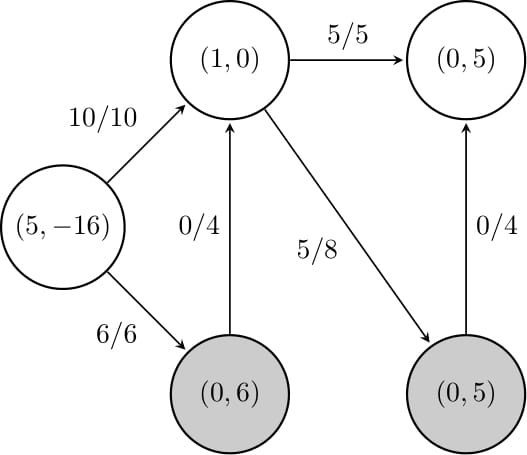
\includegraphics[scale=.358]{images/graf2-3/graf2-3-1.jpg}
  \caption{Opravili smo povišanje vozlišča $1$ in potistnili tok iz njega.}
\end{figure}

Sedaj vozlišče $1$ ni več v presežku. Naslednje vozlišče, iz katerega lahko pošljemo tok, je vozlišče $2$, vendar ga moramo najprej povišati.
Nastavimo $h(2) = 2$ in potisnemo iz njega tok $\delta = \min\{e(2), c(2,1) - f(2,1)\} = \min\{6, 4\} = 4$, s čimer bomo zasičili
povezavo $(2,1)$.

\begin{figure}[H]
  \centering
  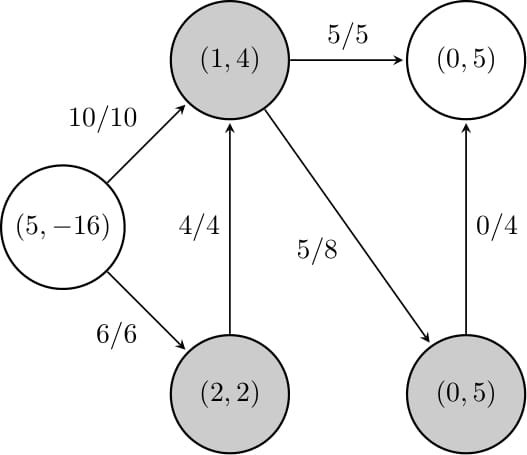
\includegraphics[scale=.358]{images/graf2-4/graf2-4-1.jpg}
  \caption{Opravili smo povišanje vozlišča $2$ in potistnili tok iz njega.}
\end{figure}

Sedaj nam ni potrebno povišati nobenega vozlišča, saj lahko potisnemo tok iz vozlišča $1$ po povezavi $(1,3)$. Potisnemo lahko
$\delta = \min \{e(1), c(1,3) - f(1,3)\} = \min \{4, 8-5\} = 3$, s čimer bomo zasičili povezavo $(1,3)$, vozlišče $1$ pa bo še vedno
ostalo v presežku.

\begin{figure}[H]
  \centering
  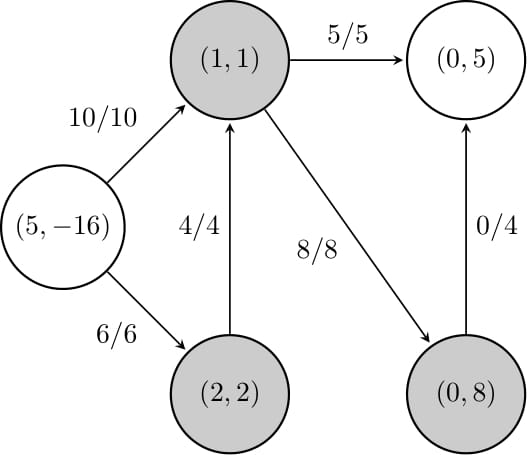
\includegraphics[scale=.358]{images/graf2-5/graf2-5-1.jpg}
  \caption{Potisnili smo tok po povezavi $(1,3)$.}
\end{figure}

Sedaj izberemo vozlišče $3$, saj ima edino še nezasičene izhodne povezave. Iz njega lahko v $t$ pošljemo $\delta = \min\{e(3), c(3,4) - f(3,4)\} = 4$ enot,
vendar ga moramo najprej povišati na višino $1$.

\begin{figure}[H]
  \centering
  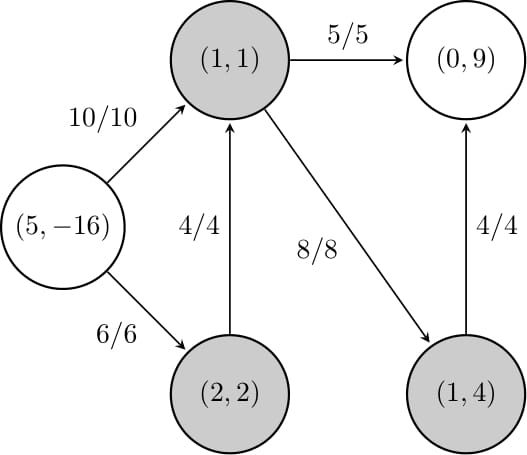
\includegraphics[scale=.358]{images/graf2-6/graf2-6-1.jpg}
  \caption{Povišali smo vozlišče $3$ in potisnili tok po povezavi $(3,4)$.}
\end{figure}

Očitno smo sedaj v $t$ dobili največ toka, kolikor ga lahko dobimo, saj je $e(t) = 9 = \sum_v (v,t)$. Vendar se na tej točki algoritem ne ustavi. Razlog za to
lahko vidimo v tem, da smo iz $s$ poslali $16$ enot, v $t$ pa prejeli le $9$ enot, kar nam nekako ni všeč, saj se je $16-9 = 7$ enot po poti izgubilo. Prav tako
imamo še vedno vozlišča v presežku, iz katerih lahko tok potisnemo. Kakor bomo videli v lemi \ref{lem:potisk_ali_povisanje}, in kakor je morda očitno, lahko na tem
vozlišču opravimo eno od operacij \texttt{POTISNI} ali \texttt{POVIŠAJ}.

Izberemo si vozlišče $3$, v katerem je trenuten presežek $4$. V vozlišče $t$ iz njega ne moremo potisniti, saj je povezava z njim zasičena. Lahko pa tok \textit{vrnemo}
v vozlišče $1$. To pravzaprav pomeni, da pošljemo tok po residualni povezavi $(3,1)$. Preden to naredimo, moramo seveda vozlišče $3$ povišati.

\begin{figure}[H]
  \centering
  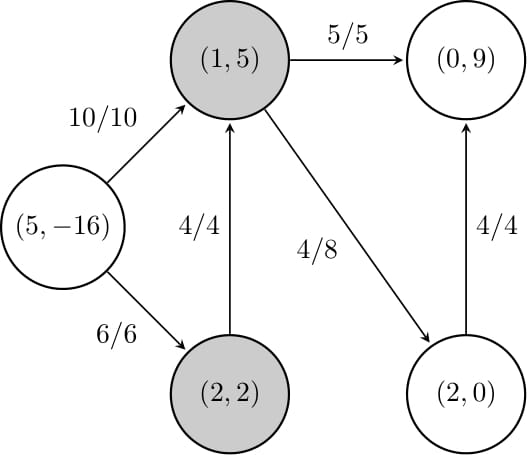
\includegraphics[scale=.358]{images/graf2-7/graf2-7-1.jpg}
  \caption{Povišali smo vozlišče $3$ in potisnili tok po residualni povezavi $(3,1)$, kar je analogno temu, da smo zmanjšali tok po povezavi $(1,3)$.}
\end{figure}

Prišli smo do najbolj zanimivega dela celega algoritma, ki morda na prvi pogled iz\-gle\-da precej smešno. Izberemo si vozlišče $1$, iz katerega bi radi
potisnili presežek. Če to želimo storiti, moramo najprej vozlišče povišati, in sicer na $\min\lbrace h(0), h(2), h(3)\rbrace + 1 = 3$. Sedaj lahko potisnemo tok po residualni
povezavi $(1,2)$ ali pa po povezavi $(1,3)$. Logično bi se nam zdelo, da toka ne bomo pošiljali nazaj v vozlišče $3$, od koder smo ga ravno dobili, ampak storili
bomo ravno to, saj želimo tok najprej poslati po originalni povezavi, šele nato po residualni. S tem bi potencialno omogočili, da pride več toka v nova vozlišča in s tem
,,bližje'' ponoru. Povišamo tako $1$ na višino $3$ in pošljemo $4$ enote nazaj v vozlišče $3$.

\begin{figure}[H]
  \centering
  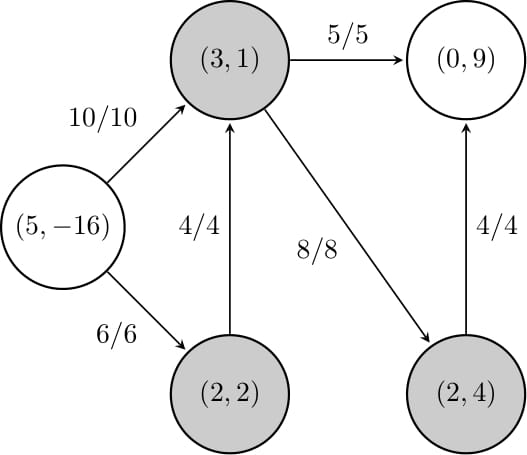
\includegraphics[scale=.358]{images/graf2-8/graf2-8-1.jpg}
  \caption{Povišali smo vozlišče $1$ in spet poslali tok v vozlišče $3$.}
  \label{fig:slika8}
\end{figure}

Kaj pa sedaj? Iz vozlišča $3$ moramo spet vrniti tok nazaj v $1$, pred tem pa še povišati višino $h(3)$ na $4$.

\begin{figure}[H]
  \centering
  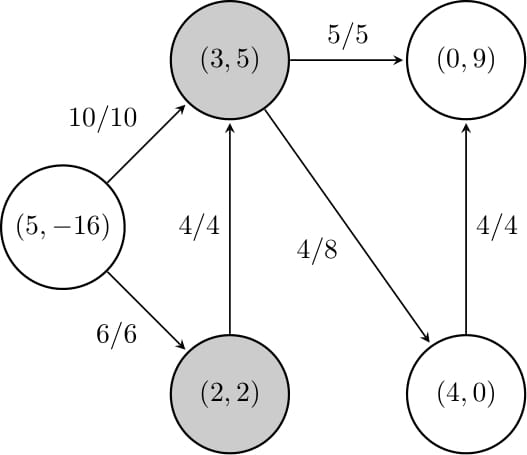
\includegraphics[scale=.358]{images/graf2-9/graf2-9-1.jpg}
  \caption{Povišali smo vozlišče $3$ in spet vrnili tok v vozlišče $1$.}
  \label{fig:slika9}
\end{figure}

V tem trenutku pa lahko končno naredimo majhen napredek, saj lahko potisnemo iz vozlišča $1$ nazaj v vozlišče $2$, namreč $h(1) > h(2)$ in obstaja povezava $(1,2)$ v residualnem
omrežju. Seveda lahko potisnemo le $\delta = \min\{e(1), f(u,v)\} = \min\{5,4\}$ $= 4$, torej bo nekaj toka še ostalo v vozlišču $1$.

\begin{figure}[H]
  \centering
  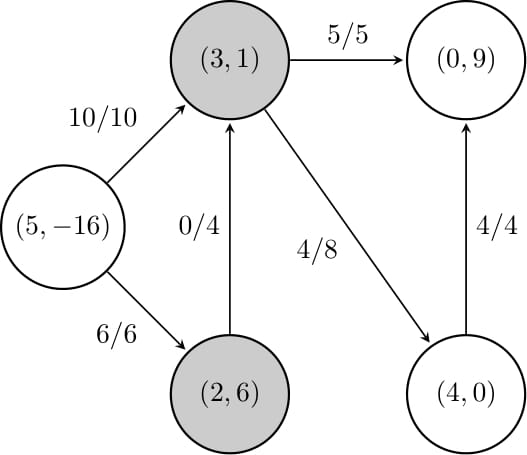
\includegraphics[scale=.358]{images/graf2-10/graf2-10-1.jpg}
  \caption{Vrnili smo tok iz vozlišča $1$ v vozlišče $2$.}
  \label{fig:slika10}
\end{figure}

Sedaj bi najraje kar vrnili $6$ enot po povezavi $(0,2)$, vendar ne moremo, saj lahko povišamo vozlišče $2$ na $\min\{h(0), h(1)\} + 1 = 4 < h(0) + 1$. Tako sedaj pošljemo
$4$ enote nazaj v vozlišče $1$ po povezavi $(2,1)$.

\begin{figure}[H]
  \centering
  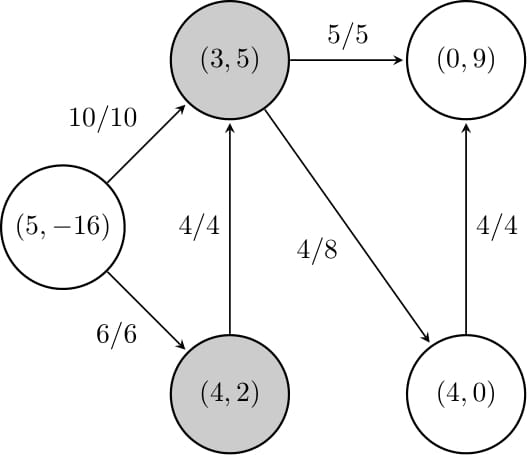
\includegraphics[scale=.358]{images/graf2-11/graf2-11-1.jpg}
  \caption{Povišamo vozlišče $2$ in spet pošljemo tok po povezavi $(2,1)$.}
\end{figure}

Podobno premislimo kot smo pri sliki \ref{fig:slika8}. Ugotovimo, da moramo povišati vozlišče $1$ na $5$ in poslati tok v vozlišče $3$.

\begin{figure}[H]
  \centering
  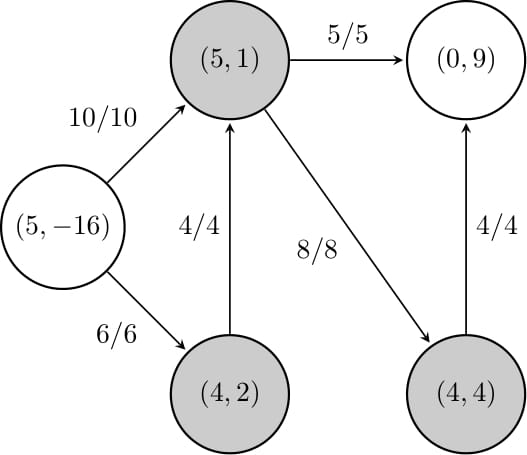
\includegraphics[scale=.358]{images/graf2-12/graf2-12-1.jpg}
  \caption{Povišamo vozlišče $1$ in spet pošljemo tok po povezavi $(1,3)$.}
\end{figure}

Razmislimo podobno kot pri sliki \ref{fig:slika9} -- povišamo vozlišče $3$ in vrnemo tok v vozlišče $1$.

\begin{figure}[H]
  \centering
  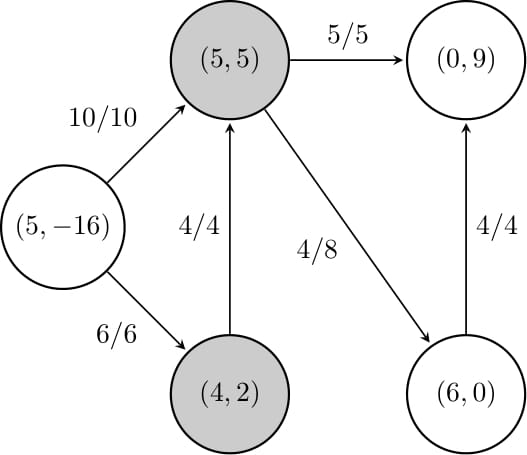
\includegraphics[scale=.358]{images/graf2-13/graf2-13-1.jpg}
  \caption{Povišamo vozlišče $3$ in vrnemo tok v vozlišče $1$.}
\end{figure}

Znašli smo se v identični situaciji kot pri sliki \ref{fig:slika9}, le višine vozlišč so drugačne. Spet lahko vrnemo tok brez povišanja
iz $1$ v $2$.

\begin{figure}[H]
  \centering
  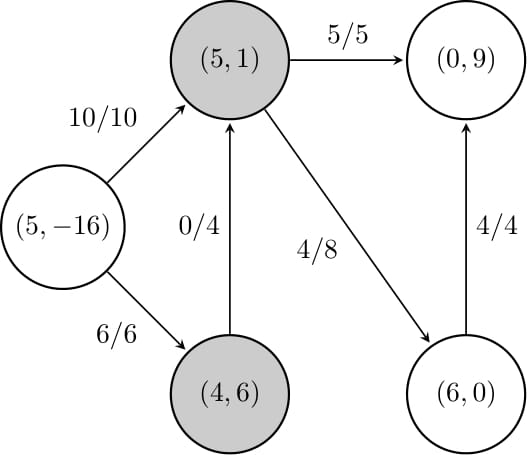
\includegraphics[scale=.358]{images/graf2-14/graf2-14-1.jpg}
  \caption{Vrnemo tok iz vozlišča $1$ v vozlišče $2$.}
\end{figure}

Povišati moramo vozlišče $2$ na $\min\{h(0), h(1)\} + 1 = 6$, vendar še ne smemo vrniti toka v $s$, saj je prosta povezava $(2,1)$, po kateri
lahko pošljemo $4$ enote. V vozlišču $2$ nam bosta potem ostali še $2$ enoti, ki pa ju končno lahko vrnemo v $s$. Znajdemo se v sledeči situaciji.

\begin{figure}[H]
  \centering
  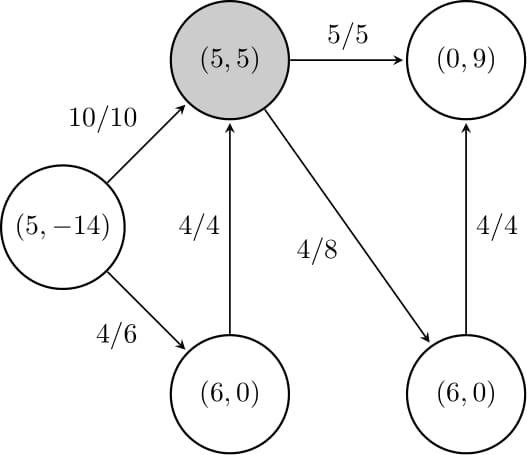
\includegraphics[scale=.358]{images/graf2-15/graf2-15-1.jpg}
  \caption{Povišamo vozlišče $2$ na $6$. Najprej pošljemo tok $4$ po originalni povezavi $(2,1)$, nato pa vrnemo tok $2$ v $s$.}
\end{figure}

Tokrat nam ne bo treba ponovno pošiljati toka iz $1$ v $3$, saj bomo vozlišče $1$ dvignili na $\min\{h(0), h(2), h(3)\} +1 = \min\{5,6,6\}+1 = 6$, kar
pa pomeni, da ne moremo potisniti v vozlišče $3$. Vrnemo torej ves tok v presežku v vozlišču $1$ v $s$ in s tem se algoritem zaključi, saj ne moremo
opraviti nobene operacije več.

\begin{figure}[H]
  \centering
  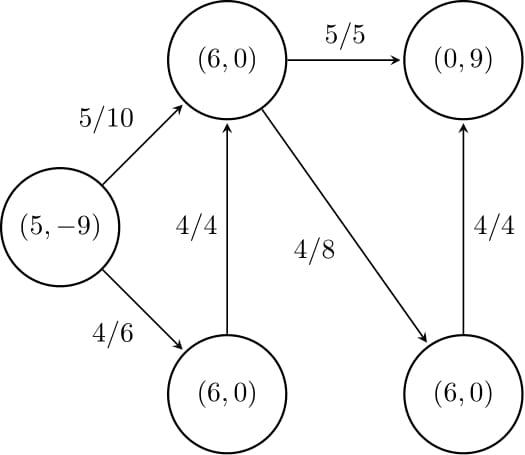
\includegraphics[scale=.358]{images/graf2-16/graf2-16-1.jpg}
  \caption{Povišamo vozlišče $1$ na $6$ in vrnemo tok $5$ v $s$. Tako izgleda naše omrežje po končanem algoritmu.}
\end{figure}

Vidimo sedaj, da po poti nismo izgubili nobene enote, saj smo jih iz $s$ poslali $9$, $9$ pa smo jih tudi prejeli v $t$. Števila $f(u,v)$, kjer je $(u,v) \in E$,
nam povedo, kolikšno količino moramo poslati po povezavi $(u,v)$, da bo pretok maksimalen.

%%%%%%%%%%%%%%%%%%%%%%%%%%%%%%%%%%%%%%%%%%%%%%%%%%%%%%%%%%%%%%%%%%%%%%%%%%%%%%%%%%%%%%%%%%%%%%%%%%%%%
%%%%%%%%%%%%%%%%%%%%%%%%%%%%%%%%%%%%%%%%%%%%%%%%%%%%%%%%%%%%%%%%%%%%%%%%%%%%%%%%%%%%%%%%%%%%%%%%%%%%%
%%%%%%%%%%%%%%%%%%%%%%%%%%%%%%%%%%%%%%%%%%%%%%%%%%%%%%%%%%%%%%%%%%%%%%%%%%%%%%%%%%%%%%%%%%%%%%%%%%%%%
%%%%%%%%%%%%%%%%%%%%%%%%%%%%%%%%%%%%%%%%%%%%%%%%%%%%%%%%%%%%%%%%%%%%%%%%%%%%%%%%%%%%%%%%%%%%%%%%%%%%%
%%%%%%%%%%%%%%%%%%%%%%%%%%%%%%%%%%%%%%%%%%%%%%%%%%%%%%%%%%%%%%%%%%%%%%%%%%%%%%%%%%%%%%%%%%%%%%%%%%%%%
%%%%%%%%%%%%%%%%%%%%%%%%%%%%%%%%%%%%%%%%%%%%%%%%%%%%%%%%%%%%%%%%%%%%%%%%%%%%%%%%%%%%%%%%%%%%%%%%%%%%%
%%%%%%%%%%%%%%%%%%%%%%%%%%%%%%%%%%%%%%%%%%%%%%%%%%%%%%%%%%%%%%%%%%%%%%%%%%%%%%%%%%%%%%%%%%%%%%%%%%%%%
%%%%%%%%%%%%%%%%%%%%%%%%%%%%%%%%%%%%%%%%%%%%%%%%%%%%%%%%%%%%%%%%%%%%%%%%%%%%%%%%%%%%%%%%%%%%%%%%%%%%%
%%%%%%%%%%%%%%%%%%%%%%%%%%%%%%%%%%%%%%%%%%%%%%%%%%%%%%%%%%%%%%%%%%%%%%%%%%%%%%%%%%%%%%%%%%%%%%%%%%%%%

\subsection{Implementacija algoritma v programskem jeziku C++}

Najprej si po\-glej\-mo idejo implementacije. Prvo vprašanje, ki se nam postavi, je, kako bomo predstavili graf. Za vsako vozlišče si moramo zapomniti njegovo višino in presežek toka, ki se v njem nahaja. Odločimo se, da bomo vozlišče predstavili s strukturo, saj bo tako koda bolj berljiva. Lahko bi sicer uporabili razred, vendar ni potrebe, lahko pa bi naredili tudi dva vektorja, enega, ki bi predstavljal višinsko funkcijo in drugega, ki bi povedal, koliko presežka toka je v vsakem izmed vozlišč. Za predstavitev grafa bomo tako uporabili vektor vozlišč in pa matriko $p\in \{0,1\}^{V \times V}$ boolovih vrednosti. Element $p_{ij}$ bo povedal, ali je povezava $(i,j)$ v grafu ali ne. Prav tako si bomo definirali dve matriki $c, f \in \N_0^{V \times V}$. Matrika $c$ bo imela na $ij$-tem mestu kapaciteto povezave $(i,j)$, matrika $f$ pa pretok preko povezave $(i,j)$.

Definirali si bomo še vrsto, v katero bomo spravljali vozlišča, ki imajo presežek toka. S tem bomo lahko do elementov, na katerih moramo opraviti operacijo potiska ali povišanja, dostopali v konstantnem času, s tem pa ne bomo uničili pravilnosti algoritma. Vzeli bomo namreč prvo vozlišče v vrsti, na njem naredili ali \texttt{POTISNI} ali \texttt{POVIŠAJ}, in ga odstranili iz vrste, če bo po opravljeni operaciji njegov presežek ničeln. Prav tako bomo na konec vrste dodali vozlišče, v katerega smo potisnili tok, če je seveda šlo za operacijo potiska. Na tej točki bomo potrebovali še vektor boolovih vrednosti, ki bo za vsako vozlišče povedal, ali smo ga že dodali med presežke. S tem se izognemo podvajanju elementov v vrsti presežkov in tako pripomoremo k hitrejšemu delovanju algoritma; in hkrati tudi pravilnejšemu, saj se lahko zgodi, da bi algoritem želel opravljati potisk ali povišanje na vozlišču, ki smo ga izpraznili, ko se je prejšnjič pojavil v vrsti.

Algoritem bomo razbili na več funkcij. Glavni funkciji bosta \texttt{potisni\_povisaj} in \texttt{potisni}, funkcija \texttt{povisaj} pa bi bila tako preprosta, da je sploh ne bomo definirali, bomo pa v komentarju v kodi zapisali, kje se zgodi.

Poglejmo si opis, kaj počne katera izmed funkcij.

\begin{itemize}
\item \texttt{potisni\_povisaj()}: Izračuna maksimalni pretok v grafu. Najprej iniciali\-zira predpretok, nato pa izvaja zanko, dokler obstaja vozlišče s presežkom. Vsakič se odloči, ali bo naredila potisk ali povišanje in potisk. Za povišanjem naredimo takoj potisk zato, da zmanjšamo število vrtljajev zanke in nam tako ni potrebno še enkrat računati najnižjega soseda, saj bo ostal isti.
\item \texttt{inicializiraj\_predpretok()}: Inicializira predpretok. Nastavi višino voz\-lišča $s$ na moč množice vozlišč. Nato potisne tok po vseh sosednjih povezavah in posodobi presežke v vozliščih. Vmes tudi doda residualno (obratno) pove\-zavo, katere kapaciteta je $0$, tok po njej pa je enak negativno predznačenemu toku, ki smo ga poslali po originalni povezavi. Če vozlišče, v katerega smo potisnili tok, ni $t$, ga dodamo med vozlišča s presežki in označimo, da je bil tja dodan.
\item \texttt{potisni(u,v)}: Potisne tok iz vozlišča $u$ v vozlišče $v$. Tok, ki ga lahko poti\-sne, je enak minimumu med presežkom v vozlišču $u$ in residualno kapaciteto povezave $(u,v)$. Če smo vozlišče $u$ izpraznili, ga odstranimo iz vrste presežkov in označimo, da ga ni več notri. Če vozlišče $v$ ni $t$ ali $s$ in še ni bilo dodano med presežke, ga dodamo.
\item \texttt{najnizji\_sosed(u)}: Poišče tisto vozlišče $v$ med sosedi $u$, ki ima najmanjšo višino in za katerega je povezava $(u,v)$ v residualnem grafu.
\item \texttt{napolni\_graf()}: Inicializira vse potrebne spremenljivke. V vektor vozlišč doda vozlišča z višino in presežkom nič. V matriko kapacitet vpiše pri\-pa\-da\-jo\-če kapacitete ter v matriki $p$ označi, katere povezave obstajajo. Funkcija predpostavi še, da ima izvir indeks $0$ in ponor indeks $|V| - 1$, torej $s = 0$ in $t = |V| - 1$.
\end{itemize}~

Oglejmo si sedaj implementacijo.

\begin{verbatim}
// Implementacija algoritma potisni-povisaj v C++

//===================================================================
//
//        KNJIZNICE IN DEFINICIJE
//
//===================================================================

#include<iostream>
#include<queue>
#include<cstdio>
#include<cstdlib>
#include<climits>

using namespace std;

// Vozlisce predstavimo s strukturo. Za vsako vozlisce si zapomnimo
// njegovo visino in presezek toka v njem.
struct Vozlisce
{
    int h, e;

    Vozlisce(int h, int e)
    {
        this->h = h;
        this->e = e;
    }
};

// Prototipi funkcij.
int potisni_povisaj();
void inicializiraj_predpretok();
void potisni(int u, int v);
int najnizji_sosed(int u);
void napolni_graf();
void sprosti_pomnilnik();

// Globalne spremenljivke.

// Množico vozlisc predstavimo z vektorjem.
vector<Vozlisce> vozlisca;

// V vrsto dajemo vozlisca, ki so v presezku. S tem lahko v
// O(1) dostopamo do naslednjega vozlisca, na katerem je potrebno
// opraviti operacijo POTISNI ali POVISAJ.
queue<int> presezki;

// V vektor shranjujemo vozlisca, ki smo jih ze dodali med
// presezke. S tem dosezemo, da se vsako vozlisce v presezkih
// pojavi kvecjemu enkrat.
vector<bool> viden;

int** c; // Matrika kapacitet povezav.
int** f; // Matrika toka.

//===================================================================
//
//        MAIN
//
//===================================================================

// Main funkcija, uporabljena za testiranje programa.
int main()
{
    // S standardnega vhoda preberi podatke o vozliscih
    // in povezavah in napolni vektorja vozlisca in povezave.
    napolni_graf();

    // Izvedi algoritem POTISNI-POVISAJ in izpisi rezultat.
    cout << "Maksimalni pretok je " << potisni_povisaj() << endl;

    // Pocistimo pomnilnik, ki smo ga porabili.
    sprosti_pomnilnik();

    return 0;
}

//===================================================================
//
//        ALGORITEM
//
//===================================================================

// Glavna funkcija algoritma potisni-povisaj. Najprej
// inicializira predpretok, potem pa izvaja operacije potiska
// in povisanja, kakor je pac potrebno. To pocne, dokler
// obstaja vozlisce s presezkom (to ne moreta biti s in t).
int potisni_povisaj()
{
    inicializiraj_predpretok();

    // Dokler ima katero izmed vozlisc presezek toka,
    // moramo opraviti ali POTISNI ali POVISAJ. Ce opravimo
    // POVISAJ, lahko takoj potem tudi potisnemo na tisto
    // vozlisce. S tem si zmanjsamo stevilo zank.
    while (presezki.size() > 0)
    {
        int u = presezki.front();
        int v = najnizji_sosed(u);

        if (vozlisca[u].h == 1 + vozlisca[v].h)
            potisni(u, v);
        else
        {
            vozlisca[u].h = vozlisca[v].h + 1; // operacija POVISAJ
            potisni(u,v);
        }
    }

    // Vrnemo presezek v vozliscu t. Lahko bi vrnili
    // tudi -presezek v vozliscu s.
    return vozlisca.back().e;
}

// Inicializira predpretok. Visino vozlisca s nastavi na
// |V|, zasici povezave iz s, doda residualne povezave
// in ce sosed ni vozlisce t, ga doda v presezke.
void inicializiraj_predpretok()
{
    vozlisca[0].h = vozlisca.size();

    for (int v = 0; v < vozlisca.size(); v++)
    {
        if (c[0][v] > 0)
        {
            // Zasici povezavo.
            f[0][v] = c[0][v];

            // Nastavi presezek v sosedu.
            vozlisca[v].e = f[0][v];

            // Doda residualno povezavo.
            f[v][0] -= f[0][v];

            // V vozliscu s posodobi oddani tok.
            vozlisca[0].e -= f[0][v];

            // Ce vozlisce ni t, ga doda v presezke.
            if (v != vozlisca.size()-1)
            {
                presezki.push(v);
                viden[v] = true;
            }
        }
    }
}

// Vrne indeks najnizjega soseda.
int najnizji_sosed(int u)
{
    int sosed;
    int min_visina = INT_MAX;

    for (int v = 0; v < vozlisca.size(); v++)
    {
        // Ce je visina soseda manjsa od trenutne najmanjse
        // visine in ce povezava ni zasicena, potem je to
        // kandidat za najnizjega soseda.
        if (vozlisca[v].h < min_visina && c[u][v] - f[u][v] > 0)
        {
            min_visina = vozlisca[v].h;
            sosed = v;
        }
    }

    return sosed;
}

// Operacija POTISNI. Potisne lahko minimum med presezkom
// v vozliscu in residualno kapaciteto povezave.
void potisni(int u, int v)
{
    int delta = min(vozlisca[u].e, c[u][v] - f[u][v]);

    // Posodobi presezek v krajiscih povezave.
    vozlisca[u].e -= delta;
    vozlisca[v].e += delta;

    // Posodobi tok prek povezave in residualne povezave.
    f[u][v] += delta;
    f[v][u] -= delta;

    // Ce smo z vozliscem opravili, ga odstranimo iz presezkov.
    if (vozlisca[u].e == 0)
    {
        presezki.pop();
        viden[u] = false;
    }

    // Ce konec povezave ni t ali s in ce vozlisce se ni v
    // presezkih, ga doda v presezke.
    if (v != vozlisca.size()-1 && v != 0 && !viden[v])
    {
        presezki.push(v);
        viden[v] = true;
    }
}

// Iz datoteke prebere podatke o stevilu vozlisc in
// povezavah. V vektor vozlisc doda vozlisca, ki jim
// nastavi visino in presezek na 0. Vsakemu vozliscu
// nato doda sosede in nastavi kapaciteto povezav.
void napolni_graf()
{
    int V;
    scanf("%d\n", &V);

    c = (int**) calloc(V, sizeof(int*));
    f = (int**) calloc(V, sizeof(int*));

    for (int i = 0; i < V; i++)
    {
        vozlisca.push_back(Vozlisce(0, 0));
        viden.push_back(false);
        c[i] = (int*) calloc(V, sizeof(int));
        f[i] = (int*) calloc(V, sizeof(int));
    }

    int u, v, kapaciteta;
    while (scanf("%d %d %d\n", &u, &v, &kapaciteta) != EOF)
    {
        c[u][v] += kapaciteta;
    }
}

// Sprosti pomnilnik, ki smo ga med izvajanjem uporabili.
void sprosti_pomnilnik()
{
    free(c);
    free(f);
}

\end{verbatim}~


Opazimo naslednjo stvar. V funkciji \texttt{potisni\_povisaj} smo zahtevali, da se pro\-gram izvaja dokler obstaja vozlišče s presežkom. Spomnimo se, da smo v psevdokodi namreč zapisali, da se mora program izvajati dokler obstaja mogoča operacija potiska ali povišanja. Da sta stvari ekvivalentni, si bomo pogledali v dokazu pravilnosti algoritma (lema \ref{lem:potisk_ali_povisanje}).



\subsection{Pravilnost delovanja algoritma}

V tem podrazdelku bomo s pomočjo lem pokazali, da tako algoritem \texttt{POTISNI-POVIŠAJ} kot tudi njegova implementacija de\-lujeta pravilno. S tem mislimo na to, da se algoritem konča in ob tem vrne pravilen rezultat, torej res pretok, ki je maksimalen. Glavni vir je knjiga \cite{clrs}.\\

Če si pogledamo, kako deluje funkcija \texttt{potisni}, vidimo, da nikjer v kodi ne uporabimo dejstva, da je razlika višine med vozliščema nujno ena. Vendar to še vseeno zahtevamo.

\begin{lema}
Naj bo $(G = (V,E), c, s, t)$ pretočno omrežje, $f\colon V \times V \rightarrow \N_0$ predpretok v $G$ in $h\colon V \rightarrow \N_0$ višinska funkcija. Potem za vsaki vozlišči $u,v \in V$ velja, da če je $h(u) > h(v) + 1$, potem povezava $(u,v)$ ni v residualnem omrežju.
\end{lema}

Ta lema nam pove, da ne obstaja residualna povezava med $u$ in $v$, če je $h(u) > h(v) + 1$. To pomeni, da če potisnemo tok v vozlišče za več kot ena nižje, ne bomo naredili nič konkretnega, kar se je preprosto prepričati.\\

% zgled

Sedaj si poglejmo obljubljeno lemo, ki nam zagotavlja pravilnost delovanja im\-plementacije in postopka, ki smo ga uporabili v zgledu. Spomnimo se namreč, da smo v implementaciji algoritem opravljali, dokler je bilo kakšno vozlišče s presežkom toka, čeprav smo v psevdokodi zapisali, da moramo algoritem opravljati, dokler je mogoča katera izmed operacij \texttt{POTISNI} in \texttt{POVIŠAJ}.

\begin{lema}[na vozlišču s presežkom lahko opravimo ali potisk ali povišanje]\label{lem:potisk_ali_povisanje}
Naj bo $(G=(V,E),c,s,t)$ pretočno omrežje, $f$ predpretok, $h$ višinska funkcija in $e\colon V \rightarrow \N_0$ funkcija, ki za vsako vozlišče pove, kolikšen je v njem presežek toka. Če ima vozlišče $u\in V$ presežek toka, torej $e(u) > 0$, potem lahko na tem vozlišču opravimo ali operacijo \texttt{POTISNI} ali operacijo \texttt{POVIŠAJ}.
\end{lema}

\begin{dokaz}
Naj ima $u$ presežek toka. Za vsako residualno povezavo $(u,v)$ velja $h(u) \leq h(v) + 1$, ker je $h$ višinska funkcija. Če ne moremo opraviti operacije \texttt{POTISNI}, potem za vse residualne povezave $(u,v)$ velja $h(u) < h(v)+1$, oziroma $h(u) \leq h(v)$. Torej lahko opravimo operacijo \texttt{POVIŠAJ}.
\end{dokaz}

Oglejmo si tri leme o višinski funkciji.

\begin{lema}[višine vozlišč se nikoli ne zmanjšajo]\label{lem:visina_ne_pada}
Med izvajanjem programa \texttt{POTISNI -POVIŠAJ} velja za vsako vozlišče $u \in V$, da se $h(u)$ nikoli ne zmanjša. Še več, vsakič, ko na $u$ opravimo povišanje, se njegova višina poveča za vsaj ena.
\end{lema}

\begin{dokaz}
Ker se višine vozlišč spreminjajo le med povišanji, je za dokaz celotne leme zadosti pokazati drugi del leme. Naj bo sedaj $u$ vozlišče, na katerem opravljamo povišanje. Torej za vse $v \in V$, za katere je $(u,v) \in E_f$, velja $h(u) \leq h(v)$. Ker to velja za vsak $v$, velja tudi \[h(u) \leq \min_{(u,v) \in E_f} h(v),\] kar pa je ekvivalentno \[h(u) < 1 + \min_{(u,v) \in E_f} h(v).\]
\end{dokaz}

\begin{lema}\label{lem:h_ostane_visinska}
Med izvajanjem programa \texttt{POTISNI-POVIŠAJ($G$,$s$)} $h$ vedno zadrži la\-stnosti višinske funkcije, opisane v definiciji \ref{def:visinska_funkcija}.
\end{lema}

\begin{dokaz}
Dokaz bomo naredili s pomočjo indukcije na število osnovnih operacij.

Po inicializaciji predpretoka je $h$ očitno višinska funkcija.

Poglejmo si najprej, kaj se zgodi med operacijo \texttt{POVIŠAJ($u$)}. \texttt{POVIŠAJ($u$)} za\-gotovi, da za vsako residualno povezavo $(u,v) \in E_f$ po opravljeni operaciji velja $h(u) \leq h(v) +1$. Vzemimo sedaj residualno povezavo, ki vstopa v $u$, recimo $(w,u) \in E_f$. Po lemi \ref{lem:visina_ne_pada} iz $h(w) \leq h(u) + 1$ pred operacijo sledi $h(w) < h(u) + 1$ po operaciji. Torej operacija \texttt{POVIŠAJ($u$)} očitno ohranja $h$ kot višinsko funkcijo.

Ostane nam pokazati še, da če je $h$ višinska funkcija pred operacijo \texttt{POTISNI($u$,$v$)}, potem je tudi po operaciji. Med to operacijo se zgodi največ ena izmed naslednjih stvari:

\begin{enumerate}
\item \textit{Dodamo residualno povezavo $(v,u)$ v $E_f$.} V tem primeru imamo $h(v) = h(u) - 1 < h(u) + 1$, torej $h$ ostane višinska funkcija.
\item \textit{Odstranimo residualno povezavo $(u,v)$ iz $E_f$.} Z odstranitvijo residualne povezave $(u,v)$ pravzaprav izgubimo zahtevo iz definicije višinske funkcije (definicija \ref{def:visinska_funkcija}), tako da $h$ na prazno ostane višinska funkcija.
\end{enumerate}

Ker vse operacije ohranjajo lastnosti višinske funkcije funkcije $h$, po principu indukcije sledi lema.
\end{dokaz}

Sledi lema, ki nam da pomembno posledico definicije višinske funkcije.

\begin{lema}\label{lem:ni_poti}
Naj bo $G=(V,E,s,t)$ pretočno omrežje, $f$ predpretok v $G$ in $h$ višinska funkcija na $V$. Potem ne obstaja pot od $s$ do $t$ v residualnem omrežju $G_f$.
\end{lema}

\begin{dokaz}
Pokažimo s pomočjo protislovja. Recimo torej, da v $G_f$ obstaja pot $p$ od $s$ do $t$, kjer je $p = \langle v_0 = s, v_1, v_2, \dotsc v_{k-1}, v_k = t\rangle$. Brez škode za splošnost lahko predpostavimo, da je $p$ enostavna pot, torej pot brez ciklov. Potem velja $k < |V|$. Ker je $p$ pot v residualnem omrežju $G_f$, za vsak $i = 0, 1, \dotsc, k-1$ velja, da je $(v_i, v_{i+1}) \in E_f$. Ker pa je $h$ višinska funkcija, za vsak $i = 0, 1, \dotsc, k-1$ velja $h(v_i) \leq h(v_{i+1}) + 1$. Od tod sledi, da velja $h(s) \leq h(t) + k$. Ampak, ker je po definiciji višinske funkcije $h(t) = 0$, dobimo $h(s) \leq k < |V|$, kar pa je v protislovju s tem, da je $h$ višinska funkcija. Veljati bi namreč moralo $h(s) = |V|$. Zaključimo, da v residualnem omrežju $G_f$ torej ne obstaja pot med $s$ in $t$.
\end{dokaz}

Manjka nam še klasični izrek iskanja maksimalnih pretokov, ki mu v angleščini pra\-vimo \textit{max-flow min-cut theorem}. Nismo se sicer spoznali s pojmom \textit{prerez omrežja}, vendar bomo izrek vseeno navedli v celoti, saj se to edino spodobi. Dokaz izreka bomo izpustili, saj je del predmeta \textit{Optimizacija} in zahteva
določena znanja, ki za algoritme tipa potisni-povišaj nimajo vrednosti, zaradi česar jih tudi nismo omenjali.

\begin{izrek}[izrek max-pretok min-prerez] \label{izr:maxflowmincut}
  Naj bo $G = (V,E)$ in $f$ pretok v omrežju $(G, c, s, t)$. Naslednje trditve so ekvivalentne.
  \begin{enumerate}
    \item $f$ je maksimalni pretok v $G$.
    \item Residualno omrežje $G_f$ ne vsebuje nobene poti od $s$ do $t$.
    \item $|f| = c(S, T)$ za nek prerez $(S,T)$ omrežja $G$.
  \end{enumerate}
\end{izrek}

Sedaj smo pridobili vso potrebno znanje, da dokažemo, da ČE se algoritem \texttt{POTISNI-POVIŠAJ} zaključi, je potem predpretok, ki ga algoritem vrne, enak ma\-ksimalnemu pretoku skozi omrežje.

\begin{izrek}
Če poženemo algoritem \texttt{POTISNI-POVIŠAJ} na danem pretočnem omrežju $(G=(V,E),c,s,t)$ in se algoritem ustavi, potem je predpretok $f$, ki ga algoritem vrne, enak maksimalnemu toku skozi dano pretočno omrežje.
\end{izrek}

\begin{dokaz}
Najprej pokažimo, da je predpretok $f$ na vsaki iteraciji zanke \texttt{DOKLER} v vrstici 2 algoritma \texttt{POTISNI-POVIŠAJ} res predpretok. Očitno je pred prvo iteracijo $f$ predpretok, saj za to poskrbi operacija \texttt{INICIALIZIRAJ\_PREDPRETOK}. Znotraj zanke \texttt{DOKLER} se lahko zgodita le dve operaciji, ali \texttt{POTISNI} ali \texttt{POVIŠAJ}. Operacija \texttt{POVIŠAJ} vpliva le na višine vozlišč in ne na vrednosti $f(u,v)$. Posledično $f$ ostane predpretok.

Med operacijo \texttt{POTISNI} pride do sprememb vrednosti $f(u,v)$. Poskrbeti moramo, da se ohranita lastnosti predpretoka:\\

\begin{enumerate}
\item Za vsako povezavo $(u,v) \in E$ velja $f(u,v) \leq c(u,v)$.
\item Za vsako vozlišče $u \in V$ velja $e(u) = \frac{1}{2}\left(\sum_{v\in V} f(v,u) - \sum_{v\in V} f(u,v)\right) \geq 0$.
\end{enumerate}~

Ker smo v vrstici 3 operacije \texttt{POTISNI} vzeli $\delta = \min\{e(u), c(u,v) - f(u,v)\}$, vidimo, da bomo ne glede na to, kaj bo minimum, uspeli zadostiti pogoju (1). Namreč, če vzamemo $c(u,v) - f(u,v)$, bomo povezavo $(u,v)$ ravno nasičili in bo po opravljeni operaciji veljalo $f(u,v) = c(u,v)$. Če pa velja $e(u) < c(u,v) - f(u,v)$, pa povezave ne bomo zasičili in tako niti ne bomo presegli njene kapacitete.

Podobno premislimo, da se ohrani lastnost (2). Če v vrstici 3 operacije \texttt{POTISNI} vzamemo $\delta = e(u)$, bomo potem v vrstici 7 zmanjšali presežek v vozlišču $u$ na nič, torej bo veljalo $e(u) = 0$. Če pa bomo vzeli $\delta = c(u,v) - f(u,v) < e(u)$, bo po opravljeni operaciji veljalo $\tilde{e}(u) = e(u) - \big(c(u,v) - f(u,v)\big) > 0$, kjer je $\tilde{e}(u)$ presežek po opravljeni operaciji. Ker $e(v)$ prištejemo pozitivno vrednost, bo po opravljeni operaciji še vedno veljalo $e(v) > 0$.\\

Ob zaključku izvajanja algoritma velja $e(u) = 0$ za vsak $u \in V\setminus \{s,t\}$. Namreč iz leme \ref{lem:potisk_ali_povisanje} in dejstva, da je $f$ po vsaki operaciji še vedno predpretok, sledi, da po zaključku ne morejo obstajati vozlišča s presežki ($s$ in $t$ namreč nikoli nista v presežku). To pomeni, da je predpretok $f$ pravzaprav tok. Lema \ref{lem:h_ostane_visinska} nam pove, da je ob zaključku algoritma $h$ še vedno višinska funkcija, od koder po lemi \ref{lem:ni_poti} sledi, da ob zaključku algoritma ni poti med $s$ in $t$ v residualnem omrežju $G_f$. Po izreku \ref{izr:maxflowmincut} (izrek o maksimalnem pretoku in minimalnem prerezu) je tako $f$ maksimalni pretok.
\end{dokaz}

S tem smo pokazali, da če se algoritem konča, dobimo pravilen rezultat. Ostane nam pokazati še, da se algoritem sploh konča. To bomo naredili v naslednjem podrazdelku, v katerem se bomo ukvarjali s časovno zahtevnostjo. Omejili bomo število operacij, ki se lahko zgodijo, in s tem pokazali, da se algoritem res konča.\\

\subsection{Časovna zahtevnost algoritma}

V tem podrazdelku bomo kot obljubljeno dokazali še, da se algoritem \texttt{POTISNI-POVIŠAJ} konča. To bomo naredili s pomočjo omejevanja števila operacij, ki se lahko zgodijo. Namesto osnovnih dveh operacij, \texttt{POTISNI} in \texttt{POVIŠAJ}, se bomo tukaj ukvarjali s tremi operacijami -- operacijo \texttt{POTISNI} bomo namreč razdelili na dve, na tisto, ki povezavo zasiči, in tisto, ki je ne. V pomoč nam bo knjiga \cite{clrs}.\\

Preden se lotimo analize časovne zahtevnosti, si poglejmo in dokažimo še eno lemo. Spomnimo se, da namreč dovolimo povezave v izvir $s$ v residualnem omrežju.\\

\begin{lema}\label{lem:enostavna_pot_s}
Naj bo $(G=(V,E),c,s,t)$ pretočno omrežje in $f$ predpretok v danem pretočnem omrežju. Potem za vsako vozlišče $x\in V$, ki je v presežku, obstaja enostavna pot od $x$ do $s$ v residualnem omrežju.
\end{lema}

\begin{dokaz}
Za vozlišče v presežku $x$ definiramo \[U = \{v : \textrm{obstaja enostavna pot od $x$ do $v$ v $G_f$}\}.\] Predpostavimo, da $s \notin U$, in pokažimo protislovje. Definirajmo še $U' = V \setminus U$. Velja torej $V = U \cup U'$. Spomnimo se še, da je $e(u) = \frac{1}{2} \left( \sum_{v\in V} f(v,u) - \sum_{v \in V} f(u,v) \right)$. Tako velja
\begin{align*}
\sum_{u \in U} e(u) &= \frac{1}{2} \sum_{u \in U} \left(\sum_{v \in V} f(v,u) - \sum_{v \in V} f(u,v)\right)\\
&= \frac{1}{2} \sum_{u \in U} \left(\left(\sum_{v \in U} f(v,u) + \sum_{v \in U'} f(v,u)\right) - \left(\sum_{v \in U} f(u,v) + \sum_{v \in U'} f(u,v)\right)\right)\\
&= \frac{1}{2} \left( \sum_{u \in U} \sum_{v \in U} f(v,u) + \sum_{u \in U} \sum_{v \in U'} f(v,u) - \sum_{u \in U} \sum_{v \in U} f(u,v) - \sum_{u \in U} \sum_{v \in U'} f(u,v) \right)\\
&= \frac{1}{2} \left(\sum_{u \in U} \sum_{v \in U'} f(v,u) - \sum_{u \in U} \sum_{v \in U'} f(u,v) \right).
\end{align*}

Zadnja enakost sledi iz dejstva, da seštevamo po povezavah, ki imajo krajišča v isti množici. Torej dobimo v vsoti tako $f(u,v)$ kot tudi $f(v,u)$. Ker velja $f(u,v) = -f(v,u)$, velja \[\sum_{u \in U} \sum_{v \in U} f(u,v) = \sum_{u \in U} \sum_{v \in U} f(v,u) = 0.\]
Vemo, da je $\sum_{u \in U} e(u) > 0$, saj $x \in U$ in $e(x) > 0$ ter $e(u) \geq 0$ za vse $u \in V$, razen $s$, za katerega smo predpostavili $s \notin U$. Torej \[ \sum_{u \in U} \sum_{v \in U'} f(v,u) - \sum_{u \in U} \sum_{v \in U'} f(u,v) > 0.\] Iz tega sledi, da obstaja povezava $(v,u)$, za katero velja $f(v,u) - f(u,v) > 0$ oziroma $f(v,u) > f(u,v)$, od koder sledi tudi $f(v,u) > 0$, kar implicira, da obstaja residualna povezava $(u, v)$. To pa pomeni, da obstaja enostavna pot od $x$ do $v$, namreč $x \rightsquigarrow u \rightarrow v$. Pot $x \rightsquigarrow u$ namreč obstaja po definiciji $U$. To pa je v protislovju z definicijo $U$.
\end{dokaz}

Z naslednjo lemo bomo omejili največjo možno višino vozlišč, njena posledica pa bo omejila skupno število opravljanj operacije \texttt{POVIŠAJ}.

\begin{lema}\label{lem:st_povisanj_vozlisca}
Naj bo $(G = (V,E),c,s,t)$ pretočno omrežje. Na koncu izvajanja algoritma \texttt{POTISNI-POVIŠAJ} na danem pretočnem omrežju za vsak $u \in V$ velja $h(u) \leq 2|V| - 1$.
\end{lema}

\begin{opomba}
Vemo, da višina vozlišč med izvajanjem \texttt{POTISNI-POVIŠAJ} ne pada. To pomeni, da je v vsakem trenutku izvajanja algoritma $h(u) \leq 2|V| - 1$ za vsak $u \in V$.
\end{opomba}

\begin{dokaz}
Višini vozlišč $s$ in $t$ se ne spreminjata. Velja $h(s) = |V| \leq 2|V| -1$ in $h(t) = 0 \leq 2|V|-1$.

Osredotočimo se torej na vozlišča $u \in V \setminus \{s,t\}$. Na začetku velja $h(u) = 0 \leq 2|V|-1$. Pokažimo, da po vsaki operaciji \texttt{POVIŠAJ} še vedno velja $h(u) \leq 2|V|-1$. Vsakič, ko povišamo vozlišče $u$, ima $u$ presežek toka. Lema \ref{lem:enostavna_pot_s} nam pove, da obstaja enostavna pot $p$ od $u$ do $s$ v residualnem grafu $G_f$. Naj bo $p = \langle v_0 = u, v_1, \dotsc, v_{k-1}, v_k = s\rangle$. Velja $k \leq |V|-1$, saj je $p$ enostavna pot. Velja tudi, da je za vsak $i = 0,1,\dotsc,k-1$ povezava $(v_i, v_{i+1}) \in E_f$. Po lemi \ref{lem:h_ostane_visinska} velja $h(v_i) = h(v_{i+1}) +1$. Če združimo te enakosti po celi poti $p$, dobimo \[h(u) = h(v_0) \leq h(v_n) + k = h(s) + k \leq h(s) + |V| - 1 = 2|V| - 1.\]
\end{dokaz}

\begin{posledica}[omejenost števila operacij \texttt{POVIŠAJ}]\label{pos:om_st_op_povisaj}
Naj bo $(G=(V,E),c,s,t)$ pretočno omrežje. Potem je število operacij \texttt{POVIŠAJ} med izvajanjem algoritma \texttt{POTISNI-POVIŠAJ} manjše od $2|V|^2$.
\end{posledica}

\begin{dokaz}
Povišamo lahko samo $|V| -2$ vozlišč; vozlišči $s$ in $t$ imata namreč ves čas isto višino. Za vozlišče $u \in V \setminus \{s,t\}$ na začetku velja $h(u) = 0$. Lema \ref{lem:st_povisanj_vozlisca} nam pove, da vozlišče $u$ ne preseže višine $2|V| - 1$ in ker višina ne pada, ga lahko povišamo največ $(2|V|-1)$-krat. Ker se to lahko zgodi za $|V|-2$ vozlišč, je število operacij \texttt{POVIŠAJ} tako navzgor omejeno z \[(|V|-2)(2|V|-1) = 2|V|^2 - 5|V| + 2 < 2|V|^2.\]
\end{dokaz}

Ostane nam pokazati še, da je tudi število operacij \texttt{POTISNI} omejeno. Kot že rečeno, bomo dokaz razbili na dva dela. Najprej bomo pokazali, da je omejeno število potiskov, ki povezavo zasičijo, potem pa bomo pokazali še, da je omejeno tudi število potiskov, ki povezave ne zasičijo.

\begin{lema}[omejenost števila operacij \texttt{POTISNI}, ki zasičijo povezavo]\label{lem:om_st_op_potisni_nas}
Naj bo $(G=(V,E),c,s,t)$ pretočno omrežje. Potem je število operacij \texttt{POTISNI}, ki povezavo zasičijo, manjše od $2|V||E|$.
\end{lema}

\begin{dokaz}
Za vsak par vozlišč $u,v \in V$ bomo prešteli, koliko potiskov, ki zasičijo povezavo, je iz $u$ v $v$ in obratno. Če kakšen tak potisk obstaja, je vsaj ena od povezav $(u,v)$ in $(v,u)$ v $E$.

Recimo, da se je zgodil potisk iz $u$ v $v$, ki zasiči povezavo $(u,v)$. Na tej točki je veljalo $h(v) = h(u) - 1$. Če želimo še kdaj potisniti iz $u$ v $v$, moramo najprej potisniti iz $v$ v $u$ nekaj toka, saj je povezava sedaj zasičena, in veljati mora $h(v) = h(u) + 1$. Ker $h(u)$ ne pada, se mora $h(v)$ povečati za vsaj $2$. Podobno premislimo, da se mora $h(u)$ povečati vsaj za $2$ med potiski iz $v$ v $u$, ki zasičijo povezavo. Spet uporabimo lemo \ref{lem:st_povisanj_vozlisca}, ki nam pove, da so višine vozlišč ves čas med $0$ in $2|V|-1$. Iz tega sledi, da se lahko $h(u)$ poveča za $2$ manj kot $|V|$-krat med delovanjem algoritma. Ker se mora med dvema potiskoma, ki zasičita povezavo, vsaj enkrat eden od $h(u)$ in $h(v)$ povečati za $2$, je tako možnih največ $2|V|$ potiskov med $u$ in $v$, ki zasičijo povezavo (lahko jih je tudi manj, če se $h(u)$ oziroma $h(v)$ povečata večkrat). Ker je povezav $|E|$, tako dobimo, da je potiskov, ki zasičijo povezavo, največ $2|V||E|$.
\end{dokaz}

\begin{lema}[omejenost števila operacij \texttt{POTISNI}, ki ne zasičijo povezave] \label{lem:om_st_op_potisni_nezas}
Naj bo $(G=(V,E),c,s,t)$ pretočno omrežje. Potem je število operacij \texttt{POTISNI}, ki ne zasičijo povezave, manjše od $4|V|^2 (|V| + |E|)$.
\end{lema}

Že pogled na zgornjo mejo nas prepriča, da bo dokaz zgornje leme težji oziroma kompleksnejši, kot dokaz prejšnjih. Pa se ga lotimo.

\begin{dokaz}
Definirajmo najprej potencial $\Phi$ kot \[\Phi = \sum_{v:e(v) > 0} h(v),\] torej kot vsoto višin vozlišč v presežku. Na začetku je $\Phi = 0$. Opazimo, da se vrednost $\Phi$ lahko spremeni po povišanju, potisku, ki zasiči povezavo, in potisku, ki povezave ne zasiči. Najprej bomo omejili, za koliko se lahko $\Phi$ poviša po potisku, ki zasiči povezavo, in povišanju. Potem bomo pokazali, da se po vsakem potisku, ki povezave ne zasiči, vrednost potenciala $\Phi$ zmanjša vsaj za $1$. To znanje bomo potem uporabili za izračun zgornje meje števila potiskov, ki povezave ne zasičijo.

Oglejmo si najprej oba načina, na katera se potencial $\Phi$ lahko poveča. Povišanje vozlišča očitno lahko poveča $\Phi$ za največ $2|V| - 1 < 2|V|$, saj po tej operaciji ostane množica, po kateri seštevamo, enaka, vozlišče pa ima po lemi \ref{lem:st_povisanj_vozlisca} lahko največjo višino $2|V|-1$, za kolikor se mu lahko tudi največ poviša. Potisk, ki zasiči povezavo $(u,v)$, lahko poveča $\Phi$ za največ $2|V|-2 < 2|V|$. Po tej operaciji se namreč množica, po kateri seštevamo, kvečjemu poveča, saj vanjo vstopi $v$, $u$ pa v njej lahko ostane ali pa ne. Če ostane, se tako lahko $\Phi$ poveča za višino vozlišča $v$, ki pa je lahko največ $2|V|-2$ (največja možna višina vozlišč je po lemi \ref{lem:st_povisanj_vozlisca} enaka $2|V| - 1$, vendar je vsaj vozlišče $u$ višje od $v$, drugače potisk ne bi bil mogoč). Če pa $u$ ne ostane v množici, torej ni več v presežku (zgodilo se je, da je veljalo $e(u) = c(u,v) - f(u,v)$), pa se $\Phi$ celo pomanjša, saj smo iz množice, po kateri seštevamo, odstranili vozlišče z večjo višino kot je višina vozlišča, ki smo ga v množico dodali.

Preostane nam obravnavati potisk, ki povezave ne zasiči. Pred potiskom je bil $u$ v presežku, vozlišče $v$ pa je lahko bilo v presežku, lahko pa tudi ne. Po operaciji $u$ ne bo več v presežku, saj pri potisku, ki povezave ne zasiči, velja $\delta = e(u)$, torej je po potisku $e(u) = 0$. Vozlišče $v$ pa je po operaciji v presežku, razen če $v = s$. To pomeni, da se je $\Phi$ zaradi operacije zmanjšal za $h(u)$, povečal pa za ali $0$ ali $h(v)$. Ker velja $h(u) - h(v) = 1$, se je $\Phi$ skupno zmanjšal za vsaj $1$.

Tako lahko iz zgornjih ugotovitev glede povečanja potenciala $\Phi$, posledice \ref{pos:om_st_op_povisaj} in leme \ref{lem:om_st_op_potisni_nas} zaključimo, da se lahko $\Phi$ poveča za največ \[(2|V|) (2|V|^2) + (2|V|) (2|V||E|) = 4|V|^2 (|V| + |E|).\] Ker je $h(u) \geq 0$ za vsak $u \in V \setminus \{s,t\}$ (vozlišči $s$ in $t$ ne moreta biti v presežku), je tudi $\Phi \geq 0$. To pomeni, da se $\Phi$ lahko zmanjša za največ $4|V|^2 (|V| + |E|)$, kar pa ravno pomeni, da je število potiskov, ki povezave ne zasičijo, enako $4|V|^2 (|V| + |E|)$.
\end{dokaz}

Sedaj pa lahko zgornje ugotovitve združimo v zaključni izrek.

\begin{izrek}[časovna zahtevnost]
Algoritem \texttt{POTISNI-POVIŠAJ} med izvajanjem na\-redi $\mathcal{O}(V^2E)$ osnovnih operacij.
\end{izrek}

\begin{dokaz}
Sledi neposredno iz posledice \ref{pos:om_st_op_povisaj} ter lem \ref{lem:om_st_op_potisni_nas} in \ref{lem:om_st_op_potisni_nezas}.
\end{dokaz}

%%%%%%%%%%%%%%%%%%%%%%%%%%%%%%%%%%%%%%%%%%%%%%%%%%%%%%%%%%%%%%%%%%%%%%%%%%%%%%%%%%%%%%%%%%%%%%%%%%%%
%%%%%%%%%%%%%%%%%%%%%%%%%%%%%%%%%%%%%%%%%%%%%%%%%%%%%%%%%%%%%%%%%%%%%%%%%%%%%%%%%%%%%%%%%%%%%%%%%%%%

\section{Primer uporabe}

%%%%%%%%%%%%%%%%%%%%%%%%%%%%%%%%%%%%%%%%%%%%%%%%%%%%%%%%%%%%%%%%%%%%%%%%%%%%%%%%%%%%%%%%%%%%%%%%%%%%
%%%%%%%%%%%%%%%%%%%%%%%%%%%%%%%%%%%%%%%%%%%%%%%%%%%%%%%%%%%%%%%%%%%%%%%%%%%%%%%%%%%%%%%%%%%%%%%%%%%%

Oglejmo si sedaj dva primera uporabe iskanja maksimalnega pretoka, s katerima se ljudje srečujejo (oziroma se srečujemo) v vsakdanjem življenju. Prvi primer bo povsem
optimizacijske narave, pri katerem bomo dobesedno iskali maksimalni pretok skozi omrežje cest, pri drugem primeru
pa bomo pravzaprav nek povsem drug problem, ki na prvi pogled izgleda čisto nepovezan s temo tega diplomskega
dela, prevedli na iskanje maksimalnih pretokov v omrežju. Idejo za primer sem dobil na Wikipediji \cite{wiki}, izpeljava in izvedba pa je lastna.

%%%%%%%%%%%%%%%%%%%%%%%%%%%%%%%%%%%%%%%%%%%%%%%%%%%%%%%%%%%%%%%%%%%%%%%%%%%%%%%%%%%%%%%%%%%%%%%%%%%%

\subsection{Problem ponudbe in povpraševanja}

Prevod imena problema iz angleščine (\textit{circulation-demand problem}) je na prvi pogled morda ne najbolj posrečen,
saj v slovenščini uporabljamo izraz ponudba in povpraševanje v kontekstu na tak način, kakor bi se v angleščini uporabljal
\textit{suply and demand}, vendar se mi zdi povsem na mestu in utemeljen.

Ta problem namreč govori o tem, da imamo $p$ podjetij, ki proizvajajo neko dobrino, ter $n$ naselij, ki to dobrino potrebujejo.
Podjetja in naselja so med seboj povezana s cestnim omrežjem, po katerem lahko prepeljemo našo dobrino. Vsaka od cest ima kapaciteto $c_i$,
ki pove, koliko enot dobrine lahko prepeljemo po njej (v neki časovni enoti). Naloga problema je najti pretok skozi omrežje pri dani funkciji
prepustnosti $c = (c_1, c_2, \dotsc, c_r)$, kjer je $r$ število vseh cest, ki zadovolji povpraševanju.\\

Recimo torej, da imamo $p$ podjetij in pišimo $\mathcal{S} = \{s_1, s_2, \dotsc, s_p\}$. Imejmo $n$ naselij in pišimo $\mathcal{T} = \{t_1, t_2, \dotsc, t_n\}$.
Označimo z $|s_i|$ količino dobrine, ki jo lahko proizvede podjetje $s_i$. Podobno označimo še $|t_i|$ količino dobrine, ki jo potrebuje naselje $t_i$.
Recimo še, da imamo dano cestno omrežje $\mathcal{C} = \{(x,y) \subseteq (\mathcal{S} \cup \mathcal{T}) \times (\mathcal{S} \cup \mathcal{T})\}$, kjer $(x,y)$ pomeni,
da imamo cesto od $x$ do $y$. Cestnemu omrežju $\mathcal{C}$ priredimo pozitivno funkcijo prepustnosti
$c = (c_1, c_2, \dotsc, c_{|\mathcal{C}|})$ za katero torej velja $c_i > 0$ za vsak $i \in \{1, 2, \dotsc, |\mathcal{C}|\}$.

Hitro ugotovimo, da gre za problem, pri katerem imamo več izvirov in več ponorov. Ker smo do sedaj obravnavali le omrežja z enim izvirom in enim
ponorom, si oglejmo naslednjo lemo.

\begin{lema}
  Pretočno omrežje $(G, c, \mathcal{S}, \mathcal{T})$, kjer je $G = (V,E)$, $\mathcal{S} = \{s_1, s_2, \dotsc, s_m\}$ množica izvirov in $\mathcal{T} = \{t_1, t_2, \dotsc, t_n\}$ množica ponorov,
  je ekvivalentno pretočnemu omrežju $(G', c', s, t)$, ki ga dobimo na naslednji način:
  \begin{align*}
    G' &= (V', E'),\\
    V' &= V \cup \{s, t\},\\
    E' &= E \cup \left\{(s, s_i) \mid s_i \in \mathcal{S}\right\} \cup \left\{(t_i, t) \mid t_i \in \mathcal{T}\right\},\\
    c'(e) &= \begin{cases} c(e) &;~~~ e \in E\\ |s_i| &;~~~ e = (s, s_i)\\ |t_i| &;~~~ e = (t_i, t) \end{cases},
  \end{align*}
  torej na način, da dodamo vozlišče $s$, ki predstavlja skupni izvir, in vozlišče $t$, ki predstavlja skupni ponor. Funkcijo prepustnosti posodobimo tako,
  da je prepustnost povezave $(s, s_i)$ enaka količini dobrine, ki jo podjetje $s_i$ lahko proizvede, in da je prepustnost povezave $(t_i, t)$ enaka povpraševanju v
  naselju $t_i$.
\end{lema}

To pomeni, da v našem primeru dodamo vozlišči $s$ in $t$, ki bosta služili kot skupen izvir in ponor. Očitno sedaj velja, da bomo zadovoljili povpraševanje v vseh naseljih natanko tedaj, ko bo
maksimalen pretok skozi dobljeno pretočno omrežje enak povpraševanju vseh naselij, torej \[ |f| = \sum_{t_i} c(t_i, t). \]

Za lažjo predstavo recimo sedaj, da imamo dve podjetji, $s_1$ in $s_2$, ter štiri nase\-lja, $t_1, t_2, t_3$ in $t_4$, s takim cestnim omrežjem in funkcijo prepustnosti, kakor kaže
naslednja slika.

\begin{figure}[H]
  \centering
  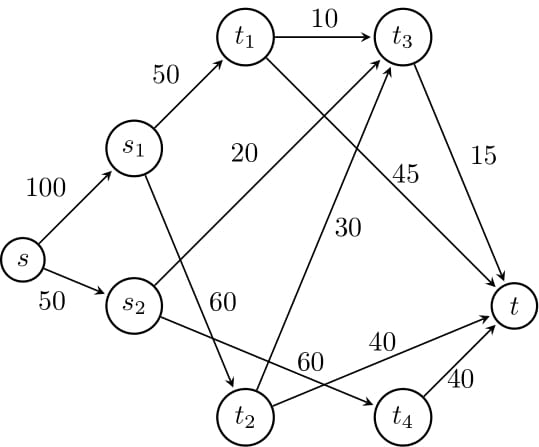
\includegraphics[scale=.358]{images/primer1-1/primer1-1-1.jpg}
  \caption{Pretočno omrežje, ki ga bomo uporabili kot zgled uporabe algoritma potisni-povišaj za problem ponudbe in povpraševanja.}
\end{figure}

Gre za preprost primer. Lahko bi se zgodilo, da bi recimo na povezavi med $t_1$ in $t_3$ bilo še neko drugo naselje, ki pa ne potrebuje te dobrine. To pomeni,
da ga iz obravnave lahko v splošnem kar izključimo. Recimo tako, da bi imeli naslednje pretočno omrežje:

\begin{figure}[H]
  \centering
  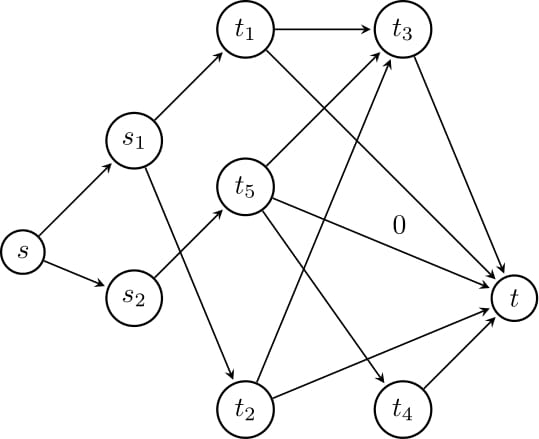
\includegraphics[scale=.358]{images/primer1-2/primer1-2-1.jpg}
  \caption{Pretočno omrežje, katerega bi se dalo poenostaviti.}
\end{figure}

To pretočno omrežje bi brez problema poenostavili na prejšnje, saj vozlišče $t_5$ očitno ne vpliva na maksimalni pretok, vendar se takim poenostavitvam v določenih primerih
rajši izognemo, saj nam vozlišča, kot so $t_5$, natančneje povedo, kje dejansko dobrina potuje. V resničnem svetu bi lahko to recimo pomenilo, da gre tovor iz Ljubljane
v Maribor preko Celja.

Vrnimo se sedaj nazaj k našemu primeru. Očitno je maksimalni pretok skozi to omrežje enak $15 + 45 + 40 + 40 = 140 = \sum_{t_i} |t_i|$, torej lahko iz podjetij $s_1$ in $s_2$
zadovoljimo potrebam vseh naselij $t_1, t_2, t_3$ in $t_4$.

\begin{figure}[H]
  \centering
  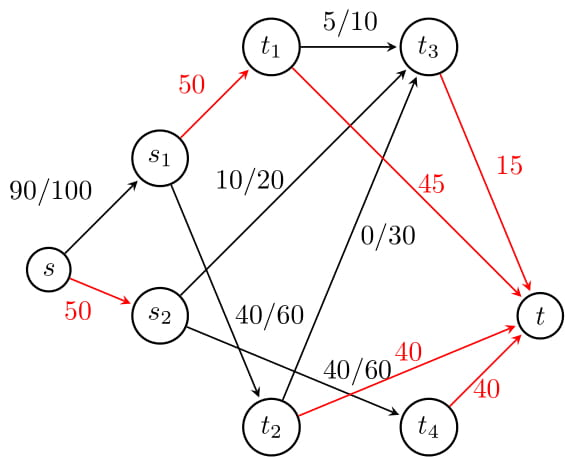
\includegraphics[scale=.358]{images/primer1-3/primer1-3-1.jpg}
  \caption{Primer maksimalnega pretoka v danem pretočnem omrežju. Povezave, obarvane rdeče, so zasičene.}
\end{figure}

%%%%%%%%%%%%%%%%%%%%%%%%%%%%%%%%%%%%%%%%%%%%%%%%%%%%%%%%%%%%%%%%%%%%%%%%%%%%%%%%%%%%%%%%%%%%

\subsection{Eliminacija ekip v baseballu}

V tem podrazdelku si bomo pogledali primer, kako nam iskanje maksimalnih pretokov pride prav v vsakdanjem življenju -- in to v primeru, ki izgleda morda povsem druge narave kakor maksimalni pretoki. Ogledali si bomo, kako lahko modeliramo pretočno omrežje, s katerim lahko določimo, ali ima ekipa v prvenstvu še možnosti za končno zmago ali izenačenje na prvem mestu.\\

Recimo, da imamo ekipe $i \in \mathcal{T} = \{ 1, 2, 3, \dotsc, n\}$, za nek $n \in \N$. Ekipa $i$ ima v nekem določenem trenutku tekom prvenstva $w_i$ zmag, do konca pa mora odigrati še $r_i$ iger. Definirajmo še $r_{ij}$ kot število iger, ki jih še mora odigrati ekipa $i$ proti ekipi $j$. Očitno velja \[r_i = \sum_{j \in \mathcal{T}\setminus\{i\}} r_{ij}.\]

Od sedaj naprej se bomo osredotočili na ekipo $x$. Poglejmo si sedaj, kako bi lahko hitro sklepali napačno. Naj bo $q$ število zmag, ki jih ima v tem trenutku vodilna ekipa. Tako bi lahko naivno sklepali, da ima naša ekipa še možnosti za zmago, če velja $w_x + r_x \geq q$. Pojasnimo, zakaj je to sklepanje napačno. Recimo, kar bomo od sedaj naprej vedno predpostavljali, da ekipa $x$ zmaga vse igre do konca prvenstva. Potem bo imela $w_x + r_x$ zmag. Recimo, da vodilna ekipa, ki ima sedaj $q$ zmag, do konca prvenstva vse igre izgubi. Naj velja $w_x + r_x \geq q$. Vendar, ker je vodilna ekipa vse igre izgubila, se lahko zgodi, da je katera izmed ostalih ekip tako morala nabrati več kot $w_x + r_x$. Oglejmo si naslednjo tabelo.

\begin{table}[H]
\centering
\caption{Trenutno stanje na lestvici, ki ga opisuje naš primer.}\vspace{3mm}
\begin{tabular}{||c||c|c||c|c|c||}
\hhline{|t:======:t|}
ekipa & $w_i$ & $r_i$ & $r_{i1}$ & $r_{i2}$ & $r_{ix}$\\ \hhline{||=||==||===||}
$1$ & $70$ & $6$ & & $3$ & $3$\\ \hhline{||-||--||---||}
$2$ & $68$ & $5$ & $3$ & & $2$\\ \hhline{||-||--||---||}
$x$ & $65$ & $5$ & $3$ & $2$ & \\ \hhline{|b:======:b|}
\end{tabular}
\end{table}

Recimo, da sedaj naša ekipa $x$ zmaga vse igre. Potem ima na koncu $w_x + r_x = 65+5=70 \geq 70 = q$ točk. Vendar morata med seboj igre odigrati tudi ekipa $1$ in $2$. Ekipa $1$ ne sme zmagati nobene igre, drugače je pred našo ekipo $x$. Torej mora proti ekipi $2$ izgubiti čisto vse $3$ igre, kar pomeni, da bo ekipa $2$ na koncu imela $68+3 = 71 > 70$ zmag. To pomeni, da kljub temu, da je $w_x + r_x \geq q$, ekipa $x$ nima več možnosti za zmago, torej je eliminirana.

Sedaj, ko smo se prepričali, da problem ni čisto trivialen, se vrnimo nazaj k splošnemu primeru, kjer imamo $n$ ekip. Recimo, da nas zanima, ali ima ekipa $n$ še možnosti za zmago. Modelirajmo naslednje pretočno omrežje:
\begin{align*}
V &= s \cup \binom{\mathcal{T} \setminus \{n\}}{2} \cup \mathcal{T} \setminus \{n\} \cup t,\\
E &= \left\{(s,(i,j)) : (i,j) \in \binom{\mathcal{T} \setminus \{n\}}{2}\right\} \cup\\
&~~~~~\cup \left\{((i,j), \alpha) : (i,j) \in \binom{\mathcal{T} \setminus \{n\}}{2} \wedge \alpha \in \{i,j\}\right\} \cup\\
&~~~~~\cup \left\{(\alpha, t) : \alpha \in \mathcal{T} \setminus \{n\}\right\},\\
c(e) &=\begin{cases}
r_{ij} &;~~~ e \in \left\{(s,(i,j)) : (i,j) \in \binom{\mathcal{T} \setminus \{n\}}{2}\right\}\\
\infty &;~~~ e \in \left\{((i,j), \alpha) : (i,j) \in \binom{\mathcal{T} \setminus \{n\}}{2} \wedge \alpha \in \{i,j\}\right\}\\
(w_n + r_n) - w_{\alpha} &;~~~ e \in \left\{(\alpha, t) : \alpha \in \mathcal{T} \setminus \{n\}\right\}
\end{cases}.
\end{align*}

To izgleda izjemno grdo in nepregledno, zato si poglejmo še shemo ravnokar definiranega pretočnega omrežja, ki je ponazorjeno na sliki \ref{fig:baseball}.

\begin{figure}
  \centering
  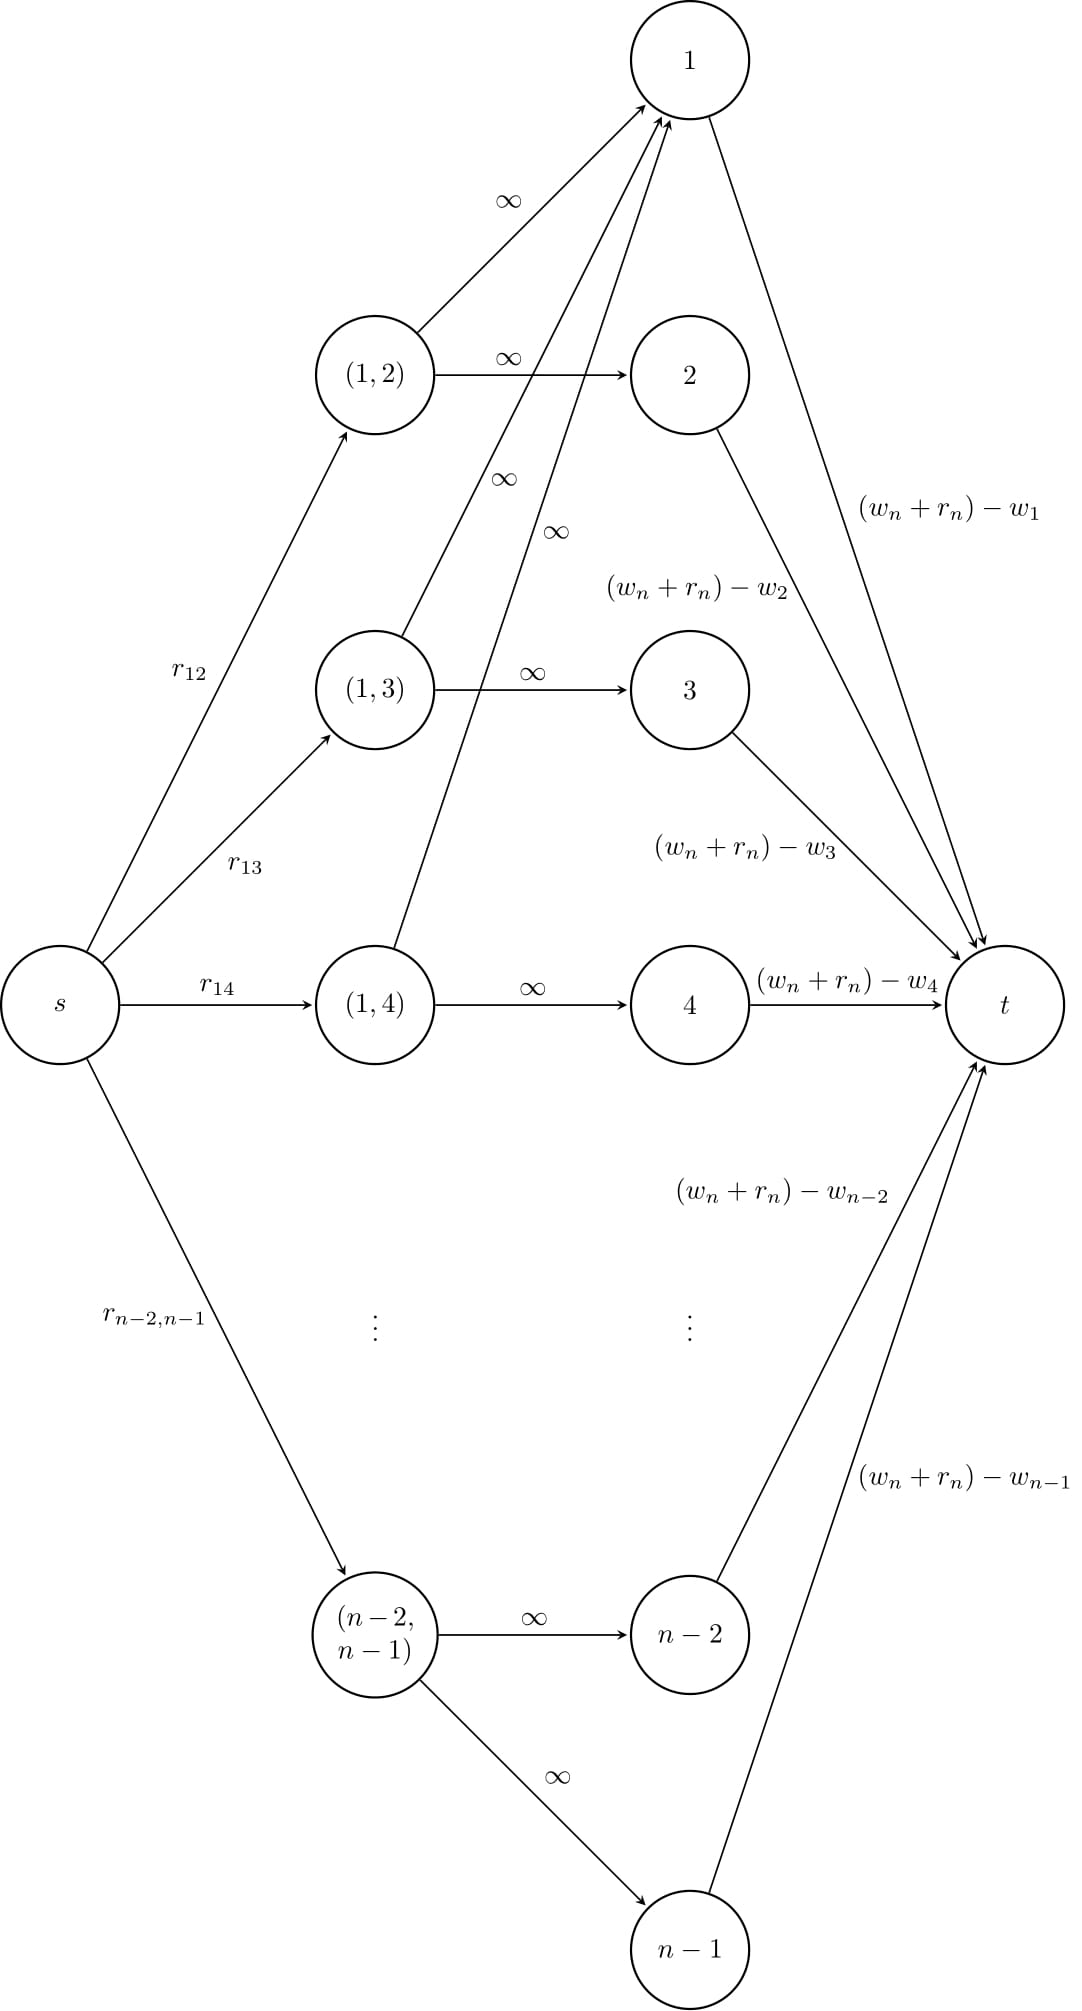
\includegraphics[scale=.32]{images/baseball1/baseball1-1.jpg}
  \caption{Omrežje, ki modelira problem eliminacije ekip v baseballu.}
  \label{fig:baseball}
\end{figure}

Opazimo, da nikjer v omrežju nimamo ekipe $n$, ravno za katero nas zanima, ali ima še možnosti za zmago. Ekipe $n$ nismo pozabili, marveč smo jo nalašč izpustili. Predpostavimo
namreč lahko, da če ima ekipa $n$ še možnosti za zmago (in ne rabi zmagati vseh preostalih iger), lahko kar rečemo, da bo zmagala vse preostale igre. S tem lahko vse, kar je povezano z ekipo $n$, izbrišemo iz omrežja.\\

Razložimo, kaj to omrežje pomeni. Vozlišče $s$ predstavlja vse igre, ki še morajo biti odigrane in ki ne vključujejo ekipe $n$. Na naslednjem nivoju imamo vozlišča oblike $(i,j)$, ki predstavljajo tekme med ekipama $i$ in $j$, ki še morajo biti odigrane.
Kot nam je že znano, $r_{ij}$ predstavlja število takih tekem. Utež na teh povezavah je torej očitno smiselna.

Na naslednjem nivoju imamo vozlišča oblike $i$, kjer vsako vozlišče predstavlja ekipo $i$. Zopet je naša ekipa $n$ izključena iz že obrazloženega razloga. Povezave, ki vstopajo v ta vozlišča, imajo omejitev neskončno, saj pravzaprav več kot $r_{ij}$ tako ali tako ne bodo mogla dobiti.

Na koncu vsa vozlišča, ki predstavljajo ekipe, povežemo v skupen ponor $t$. Uteži na povezavah, ki vstopajo v $t$, predstavljajo, koliko tekem lahko $i$-ta ekipa še zmaga, da bo naša ekipa $n$ na koncu zmagala prvenstvo. To je ravno razlika med končnim številom zmag ekipe $n$, to je $w_n + r_n$ in številom zmag,
ki jih je ekipa $i$ že dosegla, torej $w_i$.

Kako pa si lahko pomagamo s tem omrežjem pri določanju, ali ima naša ekipa še vedno možnost za končno zmago?
Označimo \[ r = \sum_{i = 1}^{n-1} r_i = \sum_{i=1}^{n-1} \sum_{j = i+1}^{n-1} r_{ij}. \] Opazimo, da je to teoretično maksimalen možen pretok v našem
pretočnem omrežju, saj več kolikor $r$ ne moremo spraviti iz izvira $s$, lahko pa se seveda zgodi, da je maksimalen pretok skozi omrežje manjši. Tako se nam porodi ideja, ki je po zgornjem razmisleku pravilna, da
ima naša ekipa $n$ še možnosti za zmago, če je vrednost maksimalnega pretoka $f$, torej $|f|$, enaka $r$.

\begin{opomba}
  Če bi nas v splošnem namesto za zadnjo ekipo, torej ekipo $n$, zanimalo, ali lahko ekipa $k \in \{1, 2, \dotsc, n\}$ zmaga prvenstvo, se stvari lotimo na povsem enak način. Ekipo $k$ izključimo iz omrežja, formula za $r$ pa se prepiše v
  \[ r = \sum_{\substack{i \in \{1, \dotsc, n\}\\i \neq k}} r_i = \sum_{\substack{i,j \in \{1, \dotsc, n\}\\ i < j\\ i, j\neq k}} r_{ij}. \]
\end{opomba}
























\newpage


\section*{Slovar strokovnih izrazov}

\geslo{potisni-povišaj}{push-relabel}
\geslo{pretok, tok}{flow}
\geslo{maksimalni pretok}{maximum flow}
\geslo{psevdopretok}{pseudoflow}
\geslo{predpretok}{preflow}
\geslo{zasičiti}{saturate}
\geslo{izvir}{source}
\geslo{ponor}{sink, terminal}


% seznam uporabljene literature
\begin{thebibliography}{99}

\bibitem{clrs}
T.H.~Cormen, C.E.~Leiserson, R.L.~Rivest in C.~Stein, \emph{Introduction to algorithms}, 3rd ed., MIT Press, Massachusetts, 2009.

\bibitem{ad}
J.~Kleinberg in E.~Tardos, \emph{Algorithm design}, Pearson Education Limited, London, 2013.

\bibitem{cpp}
S.~Meyers, \emph{Effective modern C++}, O'Reilly Media, Kalifornija, 2014.

\bibitem{aicpp}
R.~Sedgewick, \emph{Algorithms in C++}, 3rd ed., Addison-Wesley Professional, Boston, 1998.

\bibitem{uvtg}
R.J.~Wilson in J.J.~Watkins, \emph{Uvod v teorijo grafov}, Knjižnica Sigma \textbf{63}, DMFA -- založništvo, Ljubljana, 1997.

\bibitem{wiki}
\emph{Maximum flow problem}, v: Wikipedia, The Free Encyclopedia, [ogled 14.~3.~2018], dostopno na \url{https://en.wikipedia.org/wiki/Maximum_flow_problem}.

\end{thebibliography}

\end{document}
